%% 
%% Copyright 2019 Elsevier Ltd
%% 
%% This file is part of the 'CAS Bundle'.
%% --------------------------------------
%% 
%% It may be distributed under the conditions of the LaTeX Project Public
%% License, either version 1.2 of this license or (at your option) any
%% later version.  The latest version of this license is in
%%    http://www.latex-project.org/lppl.txt
%% and version 1.2 or later is part of all distributions of LaTeX
%% version 1999/12/01 or later.
%% 
%% The list of all files belonging to the 'CAS Bundle' is
%% given in the file `manifest.txt'.
%% 
%% Template article for cas-sc document class for 
%% single column output.
%\RequirePackage[undo-recent-deprecations]{expl3}
%
\RequirePackage[undo-recent-deprecations]{expl3}
%
%\RequirePackage[undo-recent-deprecations]{expl3}
%\documentclass[a4paper,fleqn,longmktitle]{cas-sc}
%\documentclass[a4paper,fleqn, twocolumn, 5p]{cas-sc}
\documentclass[a4paper,fleqn]{cas-sc}
\usepackage[version=4]{mhchem}   % For chemical formulas (e.g., \ce{HfO2})
\usepackage{amsmath}   % For advanced math symbols
%\usepackage{breqn} %package for breaking a long equation
\usepackage{siunitx} % For SI units 
\usepackage{textcomp}    % For special symbols (e.g., \textmu)
% Configure siunitx
\sisetup{
  range-phrase = \text{--},
  range-units = single,
  per-mode = fraction,
  separate-uncertainty = true
}
% Define missing units
\DeclareSIUnit{\dec}{dec}
\DeclareSIUnit{\cycle}{cycles}

\usepackage{soul} % for \hl highlighting
\usepackage{multicol}
\usepackage{array, makecell}
\usepackage{lipsum}
\usepackage{cuted}
\usepackage{mathrsfs}
\usepackage{xcolor}
\definecolor{purple}{RGB}{128,0,128}
\definecolor{magenta}{RGB}{255,0,255}

\usepackage[numbers,sort&compress]{natbib}
%\usepackage[authoryear]{natbib}
%\usepackage[authoryear,longnamesfirst]{natbib}
%%%%%%%%single-columns figure in multicolumn latex%%%%%
\usepackage[font=small,labelfont=bf]{caption}
%%%%%%%%%%%%%%%%%%%%%%%%%%%%%%%%%%%%%%%%%%%%%%%%%%%%%%%
\newenvironment{singulartabfig}
   {\par\bigskip\noindent\minipage{\columnwidth}\centering}
   {\endminipage\par\bigskip}
%%%%%%%%%%%%%%%%%%%%%%%%%%%%%%%%%%%%%%%%%%%%%%%%%%%%%%%%
\usepackage{threeparttable}
\usepackage{float}
\usepackage{makecell}  
%\usepackage{graphicx}
\usepackage{graphics}
\graphicspath{{figures/}}
\usepackage{soul}
\usepackage{color}
%https://texblog.org/2011/09/30/quick-note-on-line-spacing/
\usepackage{setspace} 
%\setstretch{4} % for custom spacing
%\setstretch{<factor>} % for custom spacing
%\onehalfspacing
%\onehalfspacing
%\doublespacing
%%%Author macros
\def\tsc#1{\csdef{#1}{\textsc{\lowercase{#1}}\xspace}}
\tsc{WGM}
\tsc{QE}
\tsc{EP}
\tsc{PMS}
\tsc{BEC}
\tsc{DE}
%%%
% Appendix equationing
% \renewcommand{\theequation}{A\arabic{equation}}

% Added for table placements
\usepackage{float}
\floatstyle{plaintop}
\restylefloat{table}
\usepackage{rotating} %for sidewaysfigure

\begin{document}
\let\WriteBookmarks\relax
\def\floatpagepagefraction{1}
\def\textpagefraction{.001}

\shorttitle{Review on Ferroelectric Materials}
% \shorttitle{}

%%%%%%%%%%%%%%%%%%%%%%%%%%%%%%%%%%%%%%%%%%%%%%%%%%%%%%%%%%%%%%%%%%%%%%%%%%%%%%%%%%%%%%%%
% ************************ Uncomment this short-Author *******************************
\shortauthors{}
% \shortauthors{S. Poudel et~al.}
%\begin{frontmatter}

%%%%%%%%%%%%%%%%%%%%%%%%%%%%%%%%%%%%%%%%%%%%%%%%%%%%%%%%%%%%%%%%%%%%%%
%%%%%Original Title cas-sc styles%%%%%%%%%%%%%%%%%%%%%%%%%%%%%%%%
%\title [mode = title]{This is a specimen $a_b$ title}                      
%\tnotemark[1,2]

%\tnotetext[1]{This document is the result of the research
%   project funded by the National Science Foundation.}

%\tnotetext[2]{The second title footnote, which is a longer text matter
%   to fill the whole text width and overflow into
%   another line in the footnotes area of the first page.}
%%%%%%%%%%%%%%%%%%%%%%%%%%%%%%%%%%%%%%%%%%%%%%%%%%%%%%%%%%%%%%%%%%%%                     
\title [mode = title]{Exploring the Potential of Ferroelectric Materials for Applications in Next-Generation Energy Technologies}
%%%%%%%%%%%%%%%%%%%%%%%%%%%%%%%%%%%%%%%%%%%%%%%%%%%%%%%%%%%%%%%%%%%%%%%%%%%%%%%%%%%%%%%%%%%%%
%%%%%Alternate titles
%%%%%%%%%%%%%%%%%%%%%%%%%%%%%%%%%%%%%%%%%%%%%%%%%%%%%%%%%%%%%%%%%%%%%%%%%%%%%%%%%%%%%%%%%%%%%
%\title [mode = title]{ Emerging Trends in Ferroelectric Materials for Next-Generation Energy Technologies}
%%%%%%%%%%%%%%%%%%%%%%%%%%%%%%%%%%%%%%%%%%%%%%%%%%%%%%%%%%%
%%%%%%%%%%%%%%%%%%%%%%%%%%%%%%%%%%%%%%%%%%%%%%%%%%%
\author[a]{Yaroslava Oliinyk}[]
%\ead{yaroslava.oliinyk11@gmail.com}
\author[b]{Mengistu Dagnaw}[]
%\ead{Mengistu.Jemberu.Dagnaw@polsl.pl/mengejembe@gmail.com}
\author[c]{Yajie Hao}[]
%\ead{25858564@edgehill.ac.uk}
%%%%%%%%%%%%%%%%%%%%%%%%%%%%%%%%%%%%%%%%%%%
\author[d]{Vytautas Stankus}[orcid=0000-0001-7702-6506]
%\ead{vytautas.stankus@ktu.lt}
%%%%%%%%%%%%%%%%%%%%%%%%%%%%%%%%%%%%%%%%%%%%%%%%%%%%%%%%%%%%%%%
\author[a]{Anil Kunwar}[orcid=0000-0003-4295-5772]
\cormark[1]
\cortext[cor1]{Corresponding author}
\ead{anil.kunwar@polsi.pl}
%%%%%%%%%%%%%%%%%%%%%%%%%%%%%%%%%%%%%%%%%%%%%%%%%%%%%%%%%%%%%%%%
%\address[a]{Department of Materials and Energy Engineering, Guizhou Institute of Technology, 550003, Guiyang, China}
%\address[b]{Guizhou Zhenhua Qunying Electrical Appliances Co.Ltd, 550018, Guiyang, China}
\address[a]{Scientific and Didactic Laboratory of Nanotechnology and Material Technologies, Faculty of Mechanical Engineering, Silesian University of Technology,44-100 Gliwice, Poland }
\address[b]{Department of Engineering Materials and Biomaterials, Faculty of Mechanical Engineering, Silesian University of Technology,44-100 Gliwice, Poland}
\address[c]{ Department of Computer Science, Edge Hill University, Ormskirk, L39 4QP, UK}
\address[d] {Department of Physics, Kaunas University of Technology, Studentu Str. 50, LT-51368 Kaunas, Lithuania }



 
\begin{abstract}
 Introduction. 
 \\ Fundamentals of ferroelectricity and ferroelectric materials.
 \\tetragonal twins in ferroelectric materials
  \\ Process-Structure-Property Relationships: Empirical Approaches
 \\ Materials Behavior Study through Experiments
 \\ Theoretical Advancements and Multiscale Computational Models.
 \\ Highlights on Energy Conversion and Storage Applications.  \\
 Conclusions about the research.

% \vspace{0.5cm}
\end{abstract}
%%%%%%%%%%%%%%%%%%%%%%%%%%%%%%%%%%%%%%%%%%%%%
%%%%%Graphical abstract has been commented%%%%

% \begin{graphicalabstract}
% %\includegraphics{figs/grabs.pdf}
% %\includegraphics{grabs.pdf}
% \centering
% \includegraphics[width=\linewidth]{figures/graphical_abstract.png}
% %\includegraphics[width=\linewidth]{graphical_abstract}
% %\includegraphics{}
% \end{graphicalabstract}

% \begin{highlights}
% \item 
% \end{highlights}

\begin{keywords}
\sep ferroelectric materials \sep gradient energy coefficients \sep multimodal energy harvesting \sep energy and AI \sep materials informatics
% Invar \sep laser welding \sep finite element analysis \sep  keyword4 \sep    keyword5 \sep keyword6
\end{keywords}
\maketitle
%%\begin{multicols}{2}
%https://www.overleaf.com/learn/latex/Multiple_columns#:~:text=Two%2Dcolumn%20documents%20can%20be,set%20of%20commands%20for%20that.
%\begin{multicols}{2}
%\begin{multicols}{2}
%https://tex.stackexchange.com/questions/196967/double-or-one-half-spacing
% \begin{doublespace}

\section{Introduction}\label{intro}
\par Ferroelectric materials have garnered significant attention due to their unique combination of piezoelectric, ferroelectric,  dielectric, pyroelectric, and electrocaloric properties. These characteristics make them highly promising for a wide range of applications, including sensors, actuators, capacitors, memory devices, solid-state refrigeration, and micro-electromechanical systems (MEMS). Their multifunctional nature continues to drive research efforts toward optimizing their performance and expanding their technological impact. \hl{to be continued...}
\par We need to present a bibliometric analysis of research work in Ferroelectric materials and their applications. Please study the user manual of VOSviewer software (\url{https://www.vosviewer.com/documentation/Manual_VOSviewer_1.6.19.pdf}), and then construct Fig.1(a) using the most important terminologies for the materials and applications. 
\par\par \hl{A good review article must have at least two tables and more than 5 non-trivial mathematical equations.}
\par \hl{AS MUCH AS IT IS POSSIBLE, WE WILL USE THE FIGURES FROM OPEN ACCESS ARTICLES + SPECIFIC}$^{*}$ \hl{SUBSCRIPTION ARTICLES (}$^{*}$ \hl{ARTICLES FROM THE PUBLISHER (ELSEVIER MAINLY AND OTHERS) WHO ALLOW THE PUBLICATION OF MORE THAN FOUR FIG. PER ARTICLE IN FREE OF CHARGE.)} 
\begin{figure}[htpb]
    \centering
    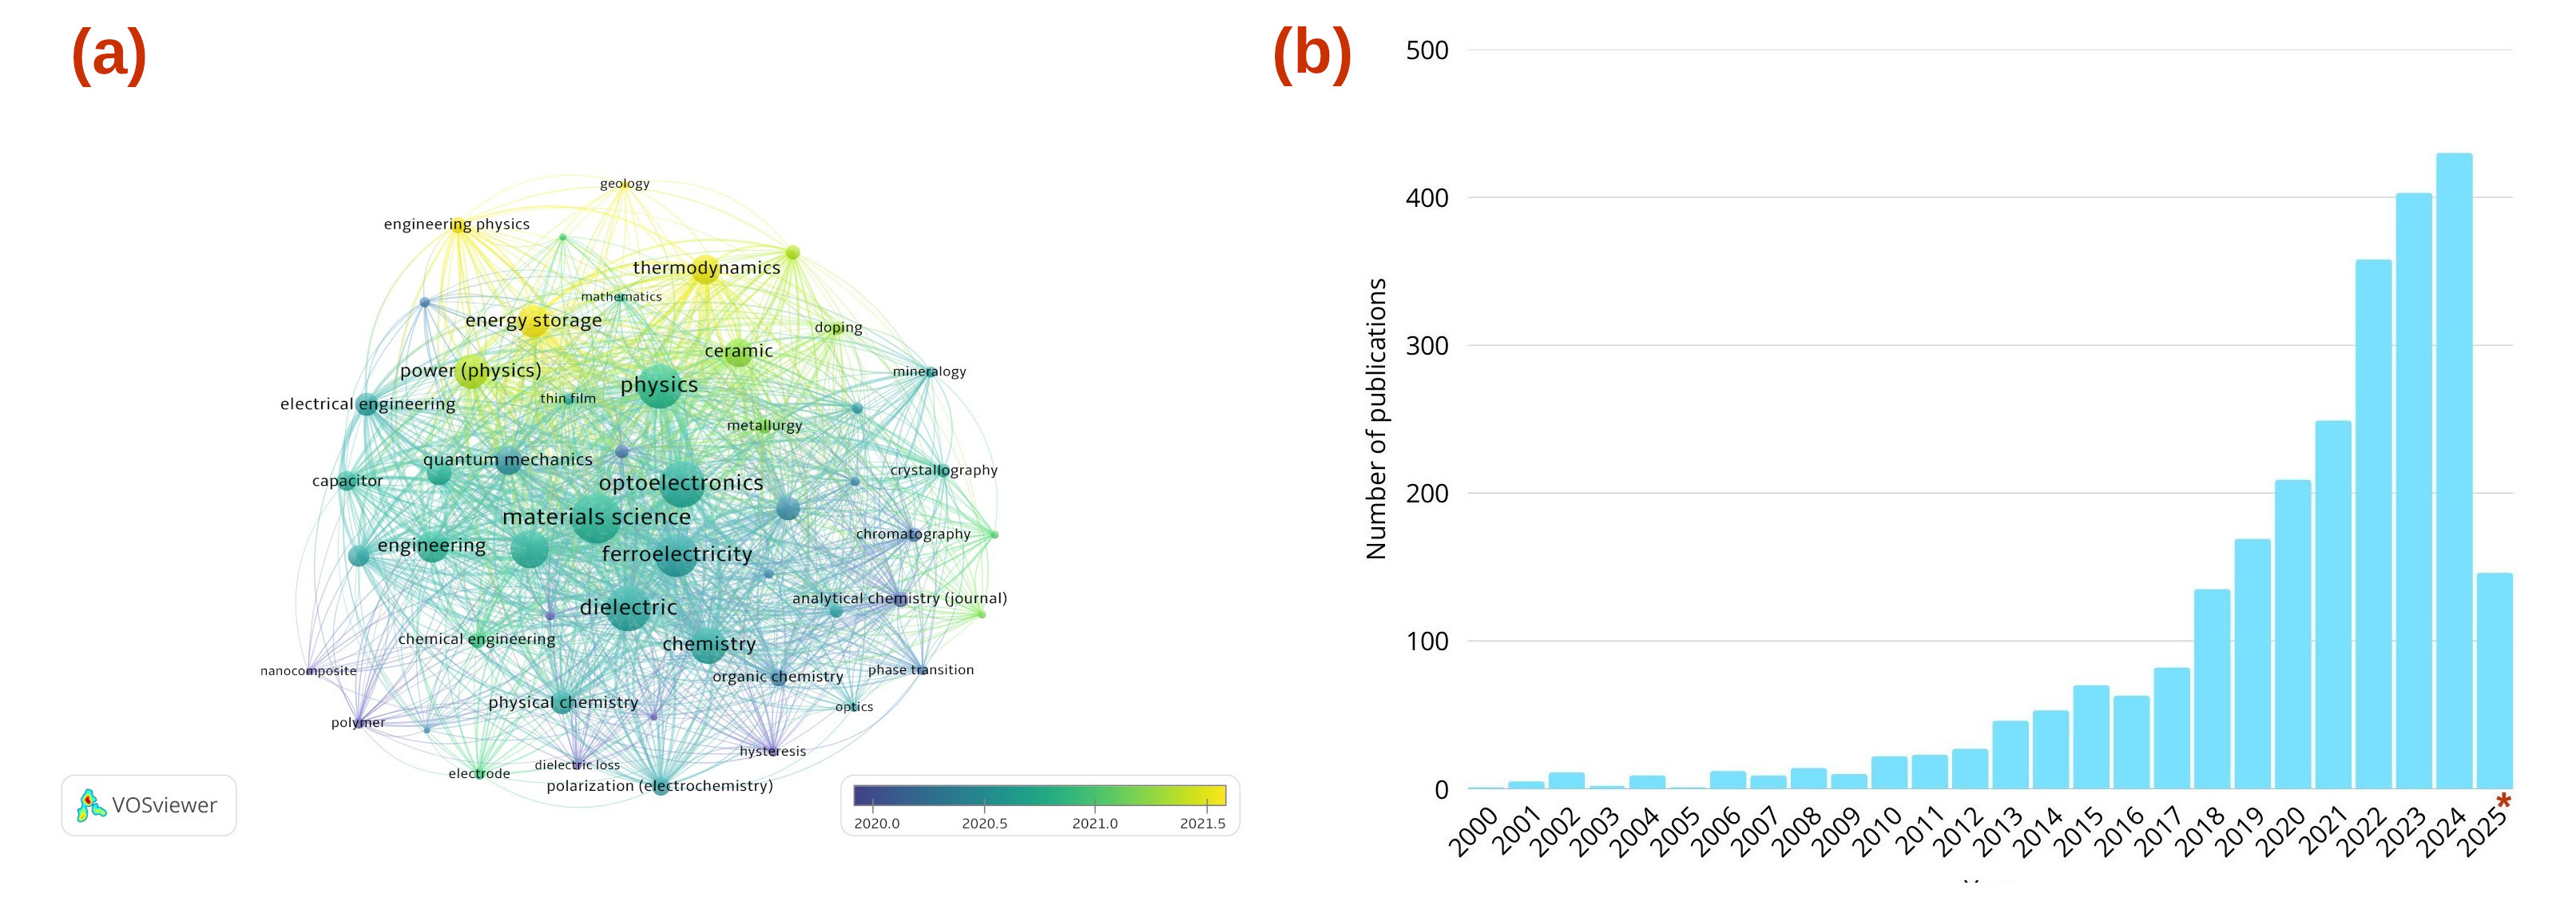
\includegraphics[width=0.84\linewidth]{Fig1.jpg}
    \caption{{a)} Bibliometric analysis of the ferroelectric materials terminologies using the VOSviewer software version {1.6.20} \cite{vanEck2010-Scientometrics}, using OpenAlex (DATABASE NAME) (date of search: {27.06.2025}. \textbf{b)} Number of publications about ferroelectrics (search words: (ferroelectricity OR "ferroelectric materials") AND ("energy storage" OR battery)) in the duration  2000-2025 (*the number of publications count for 2025 are only till the end of May). }
    \label{fig:enter-label}
\end{figure}
\section{Fundamentals of ferroelectricity and ferroelectric materials}\label{materials}
%The material used in this study is the annealed alloy 4J50 Invar, and its detailed chemical composition is listed in Table\ref{table-material1}. Sample pieces of the  4J50 Invar alloy, each  with a size (length $\times$ width $\times$ thickness) of 200 mm $\times$ 50 mm $\times$ 2 mm were selected  for welding. Before welding, the surfaces of the samples were ground with grit paper up to a grit 2000 to remove the oxidation layer, and then ultrasonically cleaned in ethanol for 10 min.
%After the cleaning procedure, two pieces of samples were assembled together for starting the joining experiments described in the following section.

%%%
\begin{table}[h]   
    \caption{\label{table-material1} This table does not belong to ferroelectric materials. Chemical composition of 4J50 Invar alloy (mass fraction,\%)}
    \centering
 \begin{tabular*}{12cm}{ccccccccc} 
%\begin{tabular*}{\textwidth}{@{\extracolsep{\fill}} llc}
   \toprule  
    Element & C & Si & Mn & S & P &Cr &Ni  & Fe       \\   
    \midrule  
    4J50  & $\leq$ 0.05   & $\leq$ 0.3     & 0.2-0.6    & $\leq$ 0.02   & $\leq$ 0.02  &-   &  36   & Balance \\
    \bottomrule 
    \end{tabular*}
    \end{table}

\subsection{fundamental concepts}\label{laser-welding-experiment}
%The pulsed laser welding equipment (JK2003SM), consisting of a Nd: YAG-pulsed laser, was used for performing the experiments. For laser welding, a butt joint is prepared from two Invar samples, as shown in the Fig.\ref{laser-welding}
%During the laser welding, pure argon gas was used through a nozzle at a 20 L/min flow rate for shielding. The parameters of Nd: YAG pulsed laser welding were tabulated in Tab.\ref{welding-parameter} 



\begin{table}[h]  
    \caption{\label{welding-parameter}  This table does not belong to ferroelectric materials. The parameters used in the Pulsed laser welding experiment. \hl{A single row is sufficient if the welding speed is the only variant.}}
    \centering
 \begin{tabular*}{13cm}{ccccc} 
%\begin{tabular*}{\textwidth}{@{\extracolsep{\fill}} llc}
   \toprule  
    \makecell{Peak Power \\(kW)}&\makecell{Pulse frequency\\ (Hz)}& \makecell{Pulse duration\\ (ms)} & \makecell{Welding speed\\ (mm/min)}  &    \makecell{Focused beam\\ diameter\\ (mm) }       \\   
    \midrule  
   45   &  15   &  2.6  &  200-300  &  1  \\
     % \midrule  
   % 45   & 15    &  2.6  &  300  &  1 \\
    \bottomrule 
    \end{tabular*}
    \end{table}

\section{Tetragonal twin structures in Ferroelectric Materials} \label{hierarchical_design}
The proper understanding of the morphology of twins in tetragonal ferroelectric materials can aid in their utilization for applications via twin engineering. \hl{In other words, the study of tetragonal twins in ferroelectric materials is vital, as their domain wall dynamics control polarization switching and energy storage efficiency, critical for applications in non-volatile memory and piezoelectric devices. Analyzing twin structures and their interactions with defects enables optimization of dielectric and mechanical properties, enhancing energy storage capacity and overall performance in ferroelectric-based technologies.} 
\par Building on this foundation, G. Arlt~\cite{Arlt1990-JMSC} established that twinning in ceramics and metals below the ferroelastic or ferroelectric phase transition temperature results from energy minimization, where homogeneous elastic energy is reduced at the expense of twin wall energy. Twin density is governed by the grain size \( d \), where the elastic energy scales as $E_{\text{elastic}}  \propto d^3 $ and the twin wall energy as $ E_{\text{twin}} \propto d^2. $ Below a critical grain size, twinning is suppressed, whereas above this threshold, the twin lamellae width follows a scaling law of $w_{\text{twin}} \propto d^{1/2}$, facilitating stress accommodation in two dimensions. For even larger grains, beyond a second critical size, more intricate interfaces emerge to relieve stress in three dimensions. This semi-quantitative model, validated using BaTiO\(_3\) ceramics, is also applicable to other materials such as YBa\(_2\)Cu\(_3\)O\(_{7-\delta}\) superconductors.
\par To demonstrate these principles in a specific material system, He et al.~\cite{HE2021116815} have investigated the morphologies of twins in tetragonal BaTiO$_3$ ferroelectrics using compatibility and energetic analysis approaches. The lamellar twin structures in these materials most commonly correspond to the \{1 1 1\} twin plane, frequently observed in pressureless-sintered BaTiO$_3$ ceramics~\cite{Wu2006-JACS}. Additionally, in the context of He et al.'s work~\cite{HE2021116815}, \{1$\overline{2}$1\} and \{2$\overline{1}$5\} twin structures also appear in BaTiO$_3$ ferroelectric materials.
\par A concrete example of this behavior is seen in the tetragonal-to-orthorhombic martensitic transformation in  BaTiO$_3$illustrated in Figures~\ref{fig:BaTiO3_crystal_slip}a--c, exemplifies the formation of twins as a mechanism to accommodate lattice distortion during phase transitions. This transformation alters the crystal symmetry, with lattice parameters of the tetragonal phase ($a_{\mathrm{t}}$, $c_{\mathrm{t}}$) transitioning to those of the orthorhombic phase ($a_{\mathrm{o}}$, $b_{\mathrm{o}}$, $c_{\mathrm{o}}$). The resulting twinning behavior is described by transformation stretch tensors, $\mathbf{U}_1$ and $\mathbf{U}_2$, which quantify the lattice distortion of martensitic variants :
\begin{equation}
\mathbf{U}_1 = 
\begin{bmatrix}
\dfrac{b_o^2 + c_o^2}{4 a_t^2} & 0 & \dfrac{b_o^2 - c_o^2}{4 a_t c_t} \\
0 & \dfrac{a_o^2}{a_t^2} & 0 \\
\dfrac{b_o^2 - c_o^2}{4 a_t c_t} & 0 & \dfrac{b_o^2 + c_o^2}{4 c_t^2}
\end{bmatrix},
\quad
\mathbf{U}_2 = 
\begin{bmatrix}
\dfrac{b_o^2 + c_o^2}{4 a_t^2} & 0 & \dfrac{c_o^2 - b_o^2}{4 a_t c_t} \\
0 & \dfrac{a_o^2}{a_t^2} & 0 \\
\dfrac{c_o^2 - b_o^2}{4 a_t c_t} & 0 & \dfrac{b_o^2 + c_o^2}{4 c_t^2}
\end{bmatrix}.
\label{eq:stretch_tensors}
\end{equation}
\par Complementing this theoretical framework, \cite{zhu2024twinning} demonstrated significant variations in lattice parameters between tetragonal and orthorhombic phases of \ce{BaTiO3} nanoparticles. Using a hydrothermal synthesis method, they reported tetragonal phase parameters as \(a_t = \SI{3.997}{\angstrom}\) and \(c_t = \SI{4.0314}{\angstrom}\). In the orthorhombic phase, the refined parameters are crucial for understanding the material's structural properties, with reported values of \(a_o = \SI{3.9874}{\angstrom}\), \(b_o = \SI{5.6751}{\angstrom}\), and \(c_o = \SI{5.6901}{\angstrom}\). These parameters are critical in modeling martensitic phase transformations, stretch tensors, and twinning behavior, providing insights into the functional characteristics of \ce{BaTiO3}, as detailed in Eq.~\ref{eq:stretch_tensors}.

\par Furthermore, the orientation relationships between twin variants and the crystallographic compatibility across twin boundaries can be analyzed using a characteristic equation:
\begin{equation}
g(f) = \det(\mathbf{C}_f - \mathbf{I}) = 0,
\label{eq:characteristic_eq}
\end{equation}
where \(\mathbf{C}_f = (\mathbf{U}_1 + f \, \mathbf{n} \otimes \mathbf{a})(\mathbf{U}_1 + f \, \mathbf{a} \otimes \mathbf{n})\), with \(\mathbf{n} \otimes \mathbf{a}\) indicating the twinning shear direction and plane. This equation predicts whether lattice mismatch can be resolved through fully compatible twins or requires localized deformation for pseudo-compatible twins.

\begin{figure}
    \centering
    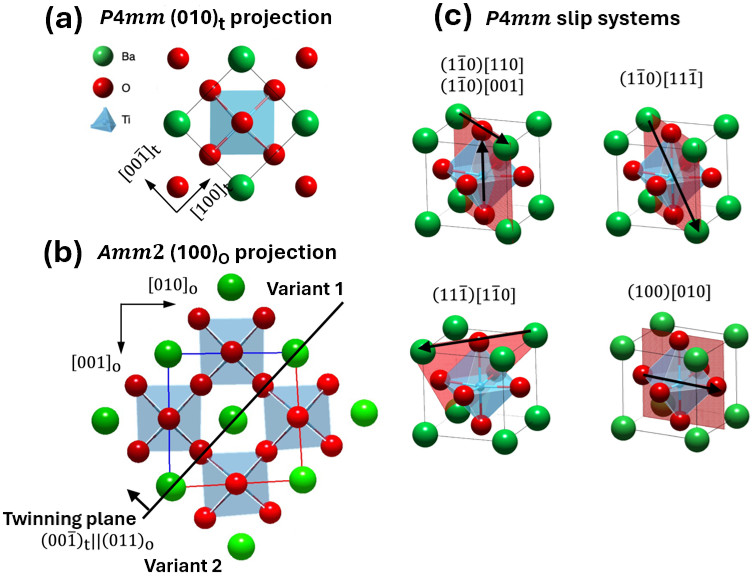
\includegraphics[width=0.8\linewidth]{figures/BaTiO3_crystal_slip}
    \caption{Crystal structure and slip systems of BaTiO$_3$ during the tetragonal-to-orthorhombic symmetries before and after martensitic phase transformation.  \textbf{(a)} Projection of the tetragonal($P4mm$) phase on the (010)$_t$ plane showing Ba, Ti, and O atomic positions. 
    \textbf{(b)} Corresponding orthorhombic($Amm2$) variants 1 and 2 projected on the (010)$_o$ plane, illustrating the twinning plane $(001)_{t} \parallel (011)_{o}$ between variants. 
    \textbf{(c)} Possible slip systems in the BaTiO$_3$ tetragonal lattice ($P4mm$) phase, indicating slip planes and directions written in terms of cubic basis relevant for plastic deformation \cite{zhu2024twinning,huang2018ferroelectric}.}
   \label{fig:BaTiO3_crystal_slip}
\end{figure}
\par Crucially, mechanical strain compatibility condition requires that the difference between the spontaneous strain tensors of adjacent twin variants, $\varepsilon^{(1)}$ and $\varepsilon^{(2)}$, satisfies $(\varepsilon^{(1)} - \varepsilon^{(2)}) \cdot \mathbf{n} = \mathbf{0}$, where $\mathbf{n}$ is the unit normal to the twin boundary. This ensures coherent, defect-free interfaces, favoring twin planes such as $\{111\}$, $\{\overline{1}21\}$, and $\{\overline{2}15\}$. More rigorously, compatibility between two variants with deformation gradients $\mathbf{A}$ and $\mathbf{B}$ demands the existence of a rotation $\mathbf{R} \in \mathrm{SO}(3)$, a vector $\mathbf{a}$, and a normal $\mathbf{n}$ such that the twinning equation $\mathbf{RB} - \mathbf{A} = \mathbf{a} \otimes \mathbf{n}$ holds, guaranteeing continuous deformation across the boundary. 
\par Supporting this, \cite{grekas2025theory} reported for potassium sodium niobate\ce{(K_{x}Na_{1-x})NbO3}(KNNex) that tetragonal stretch parameters  ($\alpha_t \approx 0.995$, $\gamma_t \approx 1.010$) yield explicit twin boundary normals $\mathbf{n}_\pm = (1/\sqrt{2})(1, \pm1, 0)$ and shear vectors: $\mathbf{a}_\pm = [2(\alpha_t - \gamma_t) / (\alpha_t^2 + \gamma_t^2)] (\pm\gamma_t, \alpha_t, 0)$, satisfying the rank-one connection. Additionally, to minimize electrostatic energy from polarization discontinuities, the polarization vectors $\mathbf{p}_A$ and $\mathbf{p}_B$ must obey $(\mathbf{p}_A - \mathbf{p}_B) \cdot \mathbf{m} = 0$, where $\mathbf{m} = (\mathbf{A}^{-\mathsf{T}}\mathbf{n}) / \|\mathbf{A}^{-\mathsf{T}}\mathbf{n}\|$ is the interface normal in the deformed configuration, ensuring pole-free interfaces. These combined mechanical and electrostatic conditions stabilize low-energy twin laminates, explaining the observed twin microstructures and crystallographic planes in tetragonal ferroelectrics, such as KNNex. 
\par The stability and formation mechanisms of ferroelectric domains, including twin domains, are further explained by the Landau–Ginzburg–Devonshire (LGD) free energy density, which incorporates contributions from polarization, elasticity, gradients, and electrostatics \cite{BHATTACHARYA2024116273}:
\begin{align} \label{lgd-batio3-ferroelectric}
    F &= \sum_{\alpha=1}^N F_{\text{bulk}}(P_i^{(\alpha)}) + \frac{1}{2} C_{ijkl} \left( \varepsilon_{ij} - \sum_{\alpha=1}^N \phi^{(\alpha)} \varepsilon_{ij}^{0(\alpha)} \right) \left( \varepsilon_{kl} - \sum_{\beta=1}^N \phi^{(\beta)} \varepsilon_{kl}^{0(\beta)} \right) \notag \\
    &\quad + \frac{1}{2} \sum_{\alpha=1}^N G_{ijkl} \frac{\partial P_i^{(\alpha)}}{\partial x_j} \frac{\partial P_k^{(\alpha)}}{\partial x_l} + \sum_{\alpha \neq \beta} \kappa_{\alpha\beta} P_i^{(\alpha)} P_i^{(\beta)} - \sum_{\alpha=1}^N E_i P_i^{(\alpha)},
\end{align}
where in Eq.~\ref{lgd-batio3-ferroelectric}, \( P_i^{(\alpha)} \) are the polarization components of the \(\alpha\)-th twin domain variant (e.g., \(\alpha = 1, 2, \ldots, N\) for \(N\) variants). The polarization vector variable-based free energy is commonly used in ferroelectric equations for modeling materials with spontaneous polarization (e.g., BaTiO$_3$). \( F_{\text{bulk}}(P_i^{(\alpha)}) \) is the bulk free energy for the \(\alpha\)-th variant.  The  \( \varepsilon_{ij}^{0(\alpha)} \) is the spontaneous strain tensor specific to the \(\alpha\)-th twin variant, reflecting its crystallographic orientation.  \(C_{ijkl}\) and \(G_{ijkl}\) respectively represent the elastic stiffness and gradient energy tensors. The gradient energy tensor governs the energy cost of domain walls between twin domains. The volume fraction of the \(\alpha\)-th twin domain (\( \phi^{(\alpha)} \)), satisfies the constraint \(\sum_{\alpha=1}^N \phi^{(\alpha)} = 1\) used to weight the contribution of each variant's strain. \( E_i \) is the applied electric field, interacting with the polarization of each variant. Carroll and Atkinson (2025) \cite{carroll2025dynamics} have applied the theoretical framework quantitatively to electron-doped perovskite ferroelectric thin films, specifically compressively strained LaAlO$_3$/SrTiO$_3$ heterostructures featuring strong out-of-plane polarization and conducting domain walls. Though twins have not been exclusively studied in their work, the material properties outlined in their work are significant for the study of ferroelectric materials with twins. Typical parameter values include a gradient energy coefficient \( g_{11} = \SI{2e-10}{\joule\cubic\meter\per\coulomb\squared} \), Landau coefficients \( a_1 = \SI{-3e8}{\joule\meter\per\coulomb\squared} \) and \( a_{11} = \SI{1.5e9}{\joule\meter\tothe{5}\per\coulomb\tothe{4}} \), which yield a saturated polarization \( P_s = \SI{0.32}{\coulomb\per\meter\squared} \) and correlation length \( \xi_0 = \SI{0.8}{\nano\meter} \). The Landau-Ginzburg-Devonshire (LGD) free energy functional captures elastic stiffness contributions through its quadratic polarization term ($\alpha P^2$), while the gradient term ($\beta|\nabla P|^2$) models the energy penalty associated with polarization inhomogeneity near domain walls. The coupling to the electric field and electron screening is governed by self-consistent solutions of the Poisson and Schrödinger equations, which describe the local electrostatics and free carrier distributions, respectively. Polarization dynamics follow the time-dependent LGD equation, $\Gamma \partial P/\partial t = -\delta F/\delta P$, where $\Gamma$ is the relaxation rate. This framework provides a quantitative description of the motion, stability, and field-driven interactions of charged ferroelectric domain walls in thin films.
\par Similarly, Peng et al.~\cite{PENG2023119297} have utilized this Physics for describing ferroelastic twin domain patterns specifically for BiVO$_4$ twin films. The free energy in their model is tailored for centrosymmetric ferroelastic materials, where twin domains arise from a tetragonal-to-monoclinic (T-M) phase transition. Bhattacharya and Zaem~\cite{BHATTACHARYA2024120039, BHATTACHARYA2024116273,BHATTACHARYA2025120702} have implemented ferroelastic Physics in their phase field simulations to study the kinetics of domain switching in yttria-stabilized zirconia (YSZ). Thus, ferroelastic equations are used to model materials that undergo spontaneous strain (e.g., BiVO$_4$, yttria-stabilized zirconia). Instead of polarization vectors, these studies~\cite{PENG2023119297,BHATTACHARYA2024116273,BHATTACHARYA2025120702} employed the structural order parameters \( \eta_i^{(\alpha)} \) in the description of free energy expression. The modified Landau--Ginzburg--Devonshire (LGD) free energy density for ferroelastic twin domain patterns in materials with spontaneous strain is given by:
\begin{align} \label{lgd-bivo4-ferroelastic}
    F &= \sum_{\alpha=1}^N F_{\text{bulk}}(\eta_i^{(\alpha)}) + \frac{1}{2} C_{ijkl} \left( \varepsilon_{ij} - \sum_{\alpha=1}^N \phi^{(\alpha)} \varepsilon_{ij}^{0(\alpha)} \right) \left( \varepsilon_{kl} - \sum_{\beta=1}^N \phi^{(\beta)} \varepsilon_{kl}^{0(\beta)} \right) \notag \\
    &\quad + \frac{1}{2} \sum_{\alpha=1}^N \beta \left( \nabla \eta_i^{(\alpha)} \right)^2 + \sum_{\alpha \neq \beta} \alpha_3 \eta_i^{(\alpha)} \eta_i^{(\beta)},
\end{align}
noting that T-YSZ exhibits small strains (0.01–0.02 along principal axes)  due to minor tetragonal deviations from cubic symmetry.
\par An important consequence of this framework is the characteristic twin wall width \( w \), which results from the balance between gradient and bulk energy contributions, following the scaling relation:
\begin{equation}
    w \approx \sqrt{\frac{G}{\alpha}},
\end{equation}
where \(G\) is an effective gradient energy coefficient, and \(\alpha\) is a Landau coefficient related to the curvature of the free energy near the spontaneous polarization state. Typically, twin walls are nanometric but may broaden under applied stress or electric fields.  In the case of epitaxial BaTiO$_3$ (BTO) thin films systematically investigated by \cite{kale2024ferroelectric}, the static and dynamic behavior of domain walls (DWs) across a wide thickness range (2--90\,nm). Their study combined piezoresponse force microscopy (PFM) with statistical scaling analysis to characterize DW motion and pinning effects. Although the domain wall width \( w \) was not explicitly derived from the analytical form \( G/\alpha \), several quantitative metrics related to wall geometry and energetics adhere to this scaling relationship. The domain wall width was estimated at \( 28 \pm 10 \) nm based on tip resolution measurements. In contrast, the Larkin length---the scale below which the wall exhibits elastic behavior---was consistently \( \sim\!1.4 \) nm across all film thicknesses. The static roughness exponent (\(\zeta\)), reflecting geometric fluctuations in domain walls, decreased slightly from \( 0.35 \) to \( 0.28 \) with reduced film thickness, suggesting stronger disorder effects. Dynamically, the creep exponent (\(\mu\)) shifted from \( 0.54 \) in thicker films (\(>\!25\) nm) to \( 0.22 \) in ultrathin films (\(<\!10\) nm), indicating a dimensional crossover from 2D sheet-like to quasi-1D string-like domain walls. These trends suggest that thinner films experience enhanced depolarization and compressive strain, likely increasing the Landau coefficient (\(\alpha\)) and narrowing the domain wall width (\(w\)), consistent with the \( \sqrt{G/\alpha} \) relationship. In contrast, thicker films exhibit reduced strain and depolarization, resulting in a decrease in \(\alpha\) and broader, more mobile domain walls. While \cite{kale2024ferroelectric} do not explicitly derive \(w\) from energy coefficients, their data corroborate the theoretical scaling \( w \propto \sqrt{G/\alpha} \).
\par Extending these principles, building on classical grain size scaling laws, recent phase-field simulations predict that the twin domain density \( \rho \) depends on grain size \(d\) and the nucleation energy barrier \(\Delta G_{\text{nuc}}\) as:
\begin{equation}
    \rho \propto d^{-\frac{1}{2}} \exp \left(- \frac{\Delta G_{\text{nuc}}}{k_B T} \right),
\end{equation}
where \(k_B\) is Boltzmann’s constant, and the nucleation barrier is given by
\begin{equation}
    \Delta G_{\text{nuc}} = \gamma_{\text{tw}} A - 2 P_s E V,
\end{equation}
Here, \(\gamma_{\text{tw}}\) is the twin wall energy density, \(A\) is the twin wall area, \(P_s\) is the spontaneous polarization, \(E\) is the applied electric field, \(V\) is the volume of the nucleated twin domain. This scaling demonstrates that smaller grain sizes promote more frequent nucleation events, owing to their higher surface-to-volume ratio and lower energy barriers under applied fields. According to recent 3D phase-field simulations~\cite{kumar20243d}, polycrystalline \ce{HfO2}--\ce{ZrO2} ferroelectric thin films (grain sizes: \SIrange{5}{50}{\nano\meter}) exhibit domain densities that adhere to the predicted scaling law. In the case of smaller grains (\SI{5}{\nano\meter}), domain density increases sharply due to stronger wall--wall coupling and stray-field interactions, which amplify the electric field contribution ($2P_s E V$). These effects, as demonstrated in the simulations, effectively lower the nucleation barrier ($\Delta G_{\text{nuc}}$), promoting higher domain densities. Notably, the number of domains per grain reduces significantly---from several to just two --- at the smallest grain sizes, consistent with the theoretical $d^{-1/2}$ dependence. The results validate thermally activated nucleation (exponentially dependent on $\Delta G_{\text{nuc}}$) and underscore grain size and field strength as key factors governing twin domain density in nanoscale ferroelectrics.
\par To quantitatively characterize twin morphologies and their energetics, recent studies have integrated mechanical compatibility conditions with Landau-Ginzburg-Devonshire (LGD) free energy models. These integrated approaches elucidate twin boundary orientations, domain wall configurations, and pathways of polar phase transitions. In particular, zhu \textit{et al.} \cite{zhu2024twinning} demonstrated that experimental studies on \ce{BaTiO3} nanopillars under uniaxial compression reveal a superelastic transformation strain consistent with theoretical predictions: $\varepsilon_{\text{trans}} = \sqrt{2}a_{\text{C}}/a_{\text{T}} - 1$, where $a_{\text{C}}$ and $a_{\text{T}}$ represent the cubic and tetragonal lattice parameters, respectively, with typical values of $\varepsilon_{\text{trans}} \approx 0.06$ matching the experimental observations within $\pm 5\%$ uncertainty, confirming the crystallographic nature of the transformation. Further, the transformation strain resolved along a loading direction $\mathbf{N}$ can be calculated by:
\begin{equation}
\epsilon_{\text{cal}}(\mathbf{N}) = \sqrt{
\mathbf{N} \cdot \mathbf{N} + 2 (\mathbf{m} \cdot \mathbf{N})(\mathbf{b} \cdot \mathbf{N}) + (\mathbf{b} \cdot \mathbf{b})(\mathbf{m} \cdot \mathbf{N})^2
} - \mathbf{N} \cdot \mathbf{N},
\end{equation}
where \(\mathbf{N}\) is the loading direction, and \(\mathbf{m}\) and \(\mathbf{b}\) represent the habit plane normal and shear vector associated with the twin interface, respectively. This relationship directly links twin geometry to macroscopic strain response, bridging microstructural morphology and functional performance.
\par Concurrently, at the nanoscale, twin nucleation enhances mechanical properties via size-dependent strengthening. Experiments on BaTiO\textsubscript{3} nanopillars reveal a yield strength scaling law of the form $\sigma_y \propto d^{-n}$, where $d$ is the characteristic dimension and $n$ is the scaling exponent typically ranging between 0.5--1.0. A more refined expression, consistent with the observed power-law scaling, incorporates strain-gradient plasticity as:
\begin{equation}
\sigma_y = \sigma_0 \left[ 1 + \left( \frac{\ell}{s} \right)^\alpha \right],
\label{eq:size_scaling}
\end{equation}
where $\sigma_0$ is the size-independent yield stress, $\ell$ is a characteristic material length scale linked to strain-gradient plasticity, $s$ is the pillar size, and $\alpha$ is the scaling exponent. This formulation captures the size-dependent strengthening effect observed at micron scales. For pillars larger than a critical size (\textasciitilde330\,nm), the data exhibit classic inverse size-scaling, characterized by a linear increase in yield strength with the inverse of pillar size consistent with  $\alpha = 1$ in the strain-gradient plasticity framework. However,  below this threshold, the yield strength saturates near \ce{BaTiO3}'s theoretical strength (\textasciitilde9\,GPa), suggesting a size-independent regime governed by slip-mediated deformation rather than twin formation. Together, these theoretical and experimental frameworks—spanning nucleation scaling, transformation strain, and yield behavior—reveal a coherent progression in understanding how twin behavior in nanoscale ferroelectrics depends on size and field.
\par Recent experimental observations by \cite{liu2025electric} using Bragg coherent diffraction imaging (BCDI) reveal domain wall dynamics in $\sim\!200\,\mathrm{nm}$ \ce{BaTiO3} nanoparticles under electric fields ($\leq\!3\,\mathrm{MV/m}$). Figure~\ref{fig:BCDI_domain_dynamics_multiplane}a--b shows a side-by-side migration model that demonstrates that domain walls primarily move at nanoparticle surfaces, where minimal strain enhances domain mobility. This surface-driven mechanism explains the higher dielectric constant in nanoscale \ce{BaTiO3} compared to bulk, where strain impedes domain motion. The lattice tetragonality ratio ($c/a$) remains stable during domain shifts, confirming distortion-free motion, quantified by:
\begin{equation} 
\frac{c}{a} = \sqrt{1 + \frac{a^2}{2 \pi} \left( \frac{\Delta \varphi_1}{\Delta x_1} - \frac{\Delta \varphi_2}{\Delta x_2} \right)}.
\end{equation}
The parameters $\Delta\varphi_{1,2}$ and $\Delta x_{1,2}$ denote the positive and negative phase slopes and domain thicknesses, respectively. The $c/a$ ratio remains nearly constant ($\sim\!1.0005$), suggesting domain wall migration dominates over lattice parameter changes \cite{liu2025electric}.
%%%%%%%%%%%%%%%%%%%%%%%%%%%%%%%%%%%%%%%%%%%%%%%%%%%%%%%%%%%%%%%%%%%%%%%%%%%%%%%%%%%%%%%%%%%
\begin{figure}
\centering
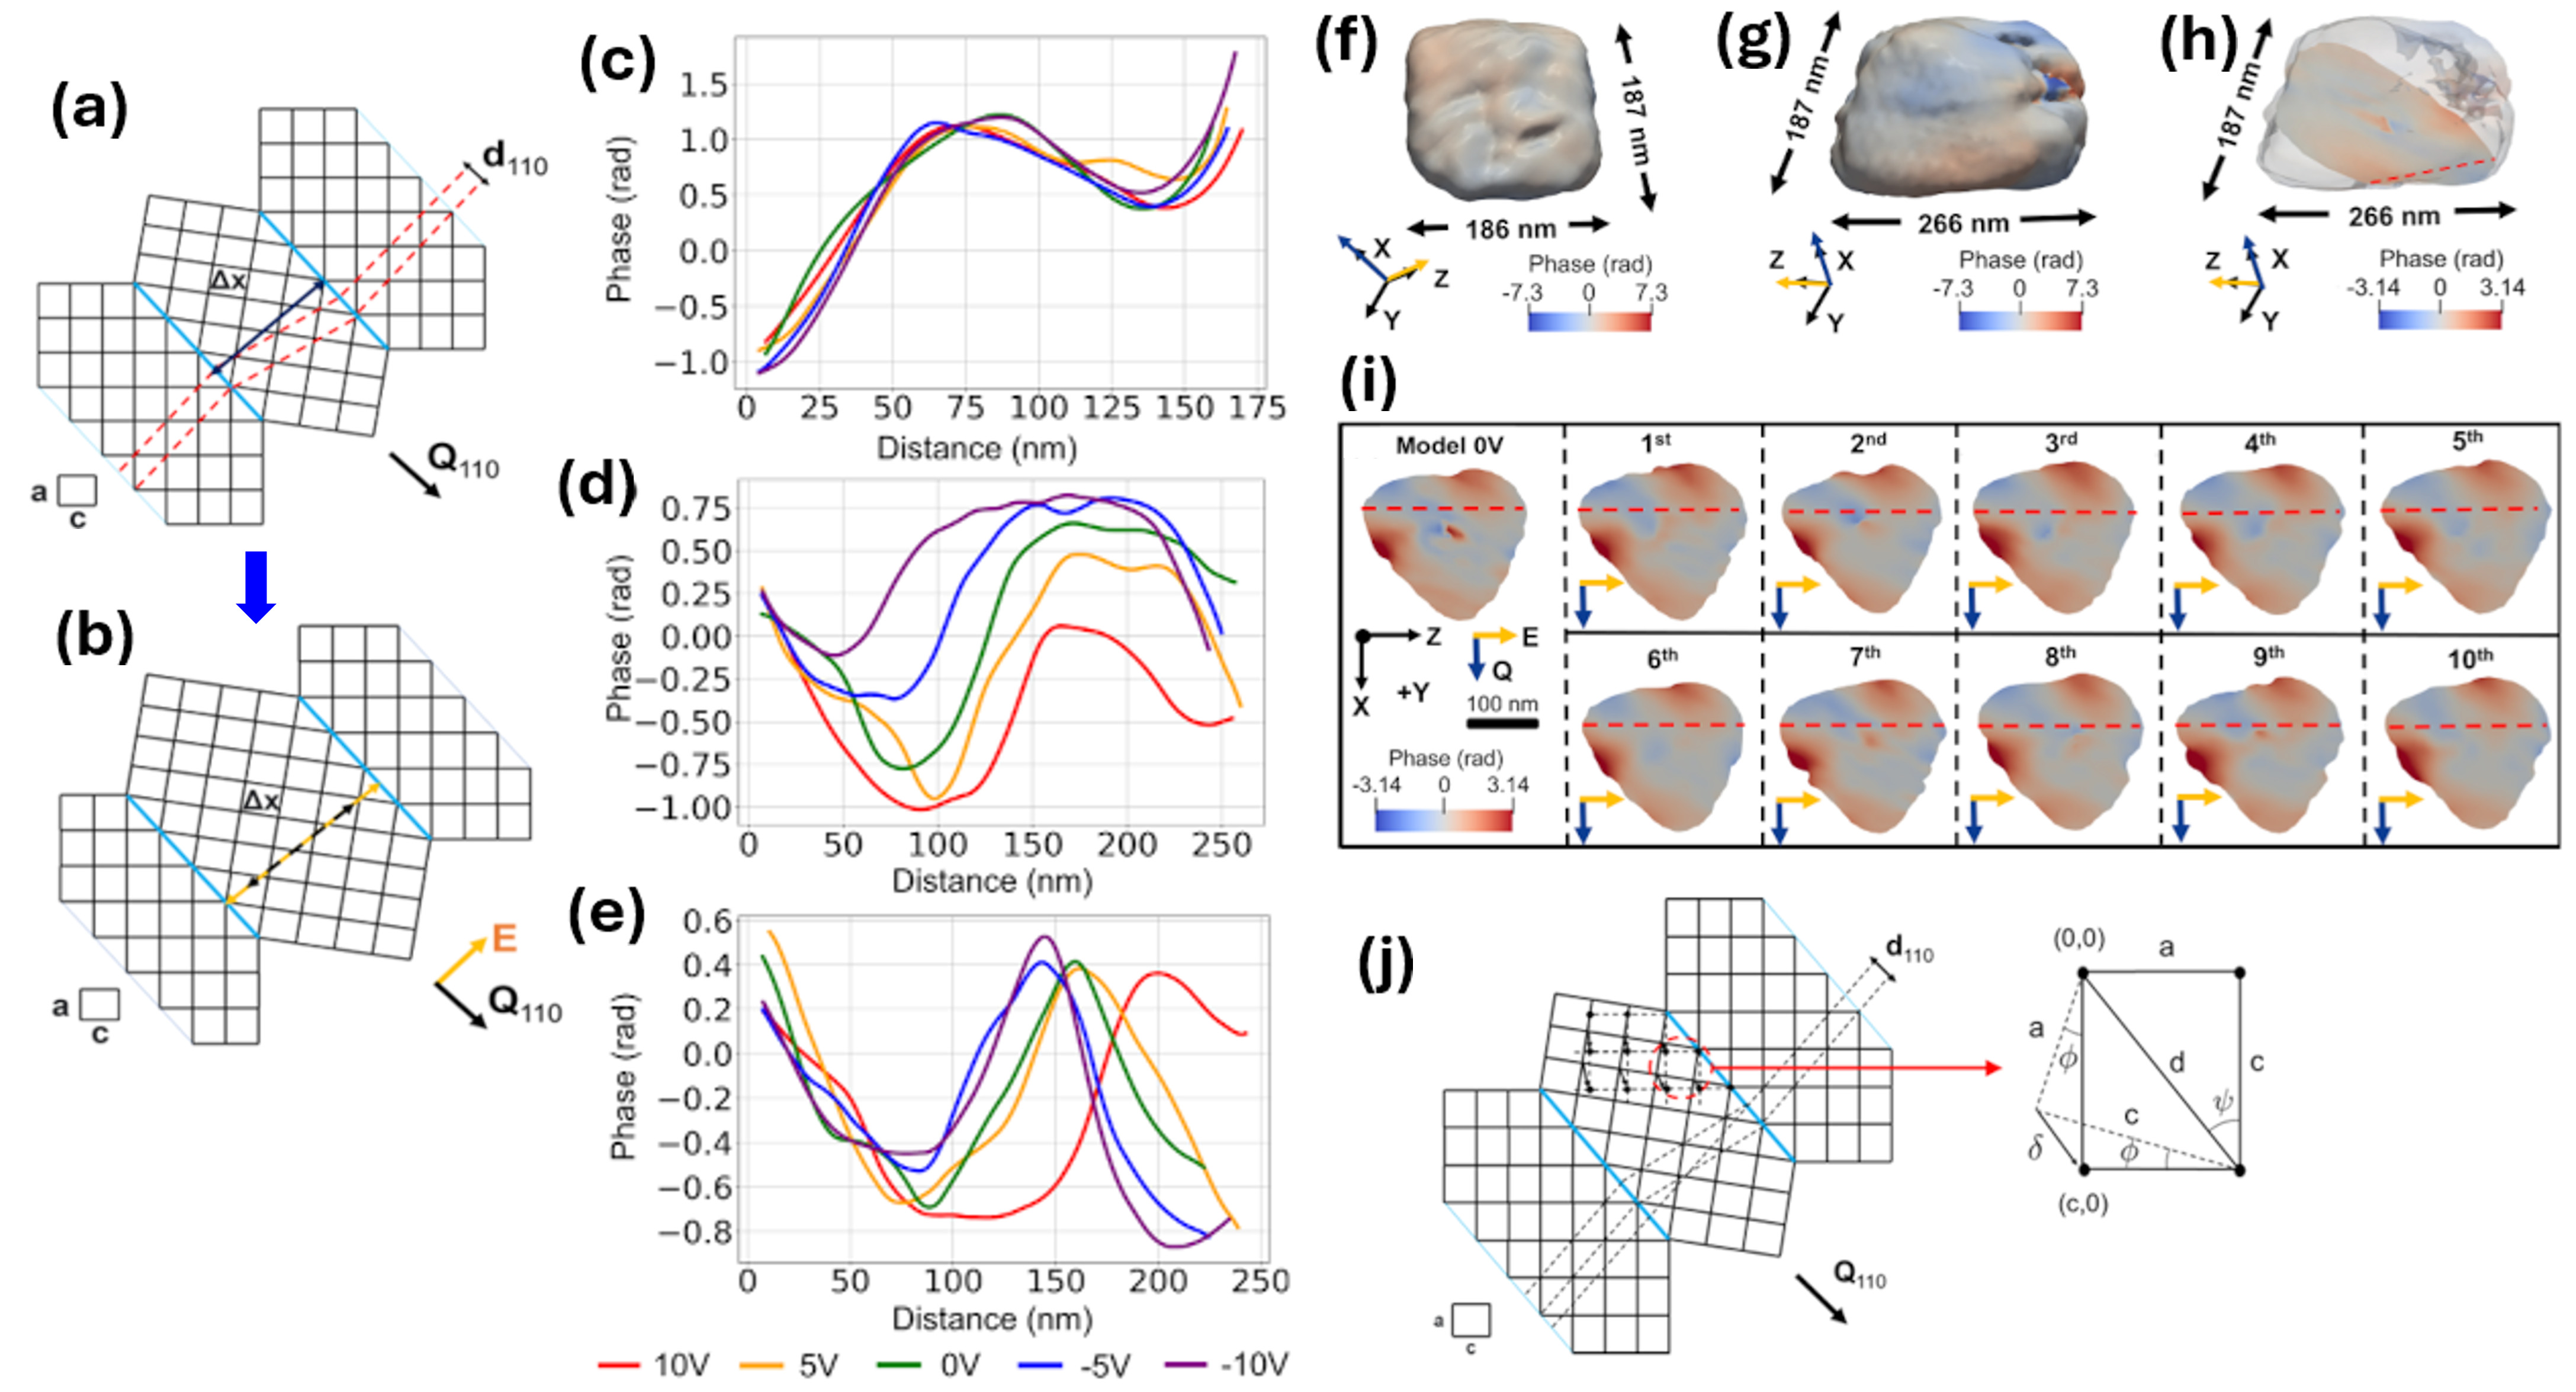
\includegraphics[width=0.95\linewidth]{figures/BCDI_domain_dynamics_multiplane}
\caption{Presents domain dynamics and structural characterization in BaTiO\(_3\) nanoparticles: \textbf{(a)} Schematic of the side-by-side domain structure in BaTiO$_3$ nanoparticles, depicting alternating \textit{a}- and \textit{c}-axis domains with lattice parameters $a$ and $c$, respectively, and domain wall spacing $\Delta x$. The vector \(\mathbf{d}_{110}\) represents the direction normal to the domain walls, aligned with the crystallographic [110] orientation, thus defining the domain wall orientation. The reciprocal lattice vector \(\mathbf{Q}_{110}\) corresponds to the (110) planes and determines the direction of lattice displacement measurements via X-ray diffraction. The reciprocal lattice vector $\mathbf{Q}_{110}$ and domain wall normal $\mathbf{d}_{110}$ are labeled. \textbf{(b)} Predicted domain wall motion under an applied electric field $\mathbf{E}$ (orange arrow), illustrating field-aligned domain expansion/contraction relative to $\mathbf{Q}_{110}$. \textbf{(c-e)} Phase line profiles along domain walls under varying applied voltages (color-coded), measured in the (c) XY ($+Z$), (d) XZ ($+Y$), and (e) YZ ($-X$) planes, reveal reversible domain wall migration and anisotropic field response. \textbf{(f-h)} 3D Bragg coherent diffraction imaging (BCDI) reconstructions (0 V) display morphology and lattice displacement phase (color scales), with cross-sectional views. \textbf{(i)} Sequential BCDI phase reconstruction slices (0 V) confirm domain structure reproducibility. \textbf{(j)} Exaggerated schematic for tetragonality ratio ($c/a$) calculation from phase domains highlights $\mathbf{d}_{110}$, lattice constants ($a$, $c$), and relevant angles \cite{liu2025electric,bednyakov2025fragmented,zhang2025ferroelectric,valecha2025thermo}.}
    \label{fig:BCDI_domain_dynamics_multiplane}
\end{figure}
%%%%%%%%%%%%%%%%%%%%%%%%%%%%%%%%%%%%%%%%%%%%%%%%%%%%%%%%%%%%%%%%%%%%%%%%%%%%%%%%%%%%%
\par Collectively, these advances establish twin engineering as a promising strategy for enhancing the mechanical strength and ductility of ferroelectric materials while preserving their functional properties. Advances in ferroelectric materials demonstrate that introducing dense ferroelastic domain (twin) structures can simultaneously enhance mechanical toughness and deformability without compromising ferroelectric performance. For instance, Chen \textit{et al.} \cite{he2022morphologies} demonstrated BaTiO\textsubscript{3}-based relaxor ceramics with an ultrahigh energy-storage density ($\sim$9.04\,J/cm\textsuperscript{3}), exceptional mechanical hardness ($\sim$9.7\,GPa), and high compressive strength ($\sim$500\,MPa). This performance synergy arises from solid-solution strengthening, grain-boundary engineering, and twin-boundary effects. Notably, the system retained its dielectric energy storage capability despite enhanced mechanical robustness. Similarly, Chu \textit{et al.} \cite{chu2023superelastic} showed that \ce{BaTiO3} micropillars exhibit ferroelastic twin-domain switching with superelastic behavior, sustaining over \(10^8\) cycles without functional degradation or structural failure. This performance combines exceptional energy dissipation (large hysteresis) with remarkable durability. The superelastic fatigue resistance stems from twin-wall motion, which accommodates strain at low stress, conferring metal-like resilience to an otherwise brittle ferroelectric ceramic. Finally, Zhang \textit{et al.} \cite{zhang2025theoretical} developed theoretical models to predict the mode~I fracture toughness ($K_{\mathrm{Ic}}$) and fracture strength ($\sigma_{\mathrm{F}}$) of ferroelectric ceramics under applied electric fields. Based on Li's Principle of Energy Equivalence, also known as the mass-energy equivalence, their framework accounts for energy dissipation from domain switching near crack tips. For $\mathrm{BaTiO_3}$ and $\mathrm{PZT}$ ceramics, $K_{\mathrm{Ic}}$ increases by $\sim\!45\%$ (to $1.1\,\mathrm{MPa\cdot m^{1/2}}$) when the electric field aligns with the crack but decreases under perpendicular fields. Fracture strength exceeds $200\,\mathrm{MPa}$ in $\mathrm{BaTiO_3}$ at optimal field orientations. The models agree with experimental data, demonstrating that domain switching enhances mechanical performance without degrading ferroelectric properties. This work provides a quantitative basis for designing ferroelectrics under electromechanical loads.

%%%%%%%%%%%%%%%%%%%%%%%%%%%%%%%%%%%%%%%%%%%%%%%%%%%%%%%%%%%%%%%%%%%%%%%%%%%
%\begin{figure}
%\centering
%\includegraphics[width=0.95\linewidth]{figures/Fig-psp.jpg}
%\caption{\hl{The first figure (a) must include a schematic figure to show the correlation between PSP and performance if there are works related to it. The style can be chosen among the best among (a)-(f). The figures from (b)-(f) must contain works from reference papers that highlight one, both, or all of PS, SP, and PSP..}}
%    \label{figure-PSP}
%\end{figure}
%%%%%%%%%%%%%%%%%%%%%%%%%%%%%%%%%%%%%%%%%%%%%%%%%%%%%%%%%%%%%%%%%%%%%%%%%%%%%%%%
% Content of the caption: \textbf{Processing:} Enhanced packing density and reduced activation energy ($Q$) are achieved through a bimodal powder compaction route using 200\,nm and 80\,nm \ce{BaTiO3} particles. Increased densification yields a sintered ceramic with 92\% relative density. \textbf{Structure:} The tetragonal crystal structure is characterized by off-center displacement of \ce{Ti^4+} ions within \ce{TiO6} octahedra. Spontaneous symmetry breaking below the Curie temperature ($T_{\mathrm{c}}$) enables ferroelectricity and domain formation. \textbf{Properties:} Directional elastic coupling across crystallographic orientations is visualized by the anisotropic 3D surface of Poisson's ratio ($\nu_{ij}$). This elastic anisotropy governs mechanical-electrical feedback mechanisms critical for domain wall behavior and device energy efficiency. \textbf{Performance:} Functional energy behavior is quantified by the polarization--electric field ($P$--$E$) hysteresis loop. The red hatched area indicates the recoverable energy storage density; energy loss corresponds to the loop area. Application suitability for energy storage, sensors, and actuators is defined by remnant polarization ($P_{\mathrm{r}}$), maximum polarization ($P_{\mathrm{max}}$), and coercive field ($E_{\mathrm{c}}$). This schematic demonstrates the directional interdependencies within the PSPP framework, enabling inverse design where performance targets guide property selection and processing optimization.
%%%%%%%%%%%%%%%%%%%%%%%%%%%%%%%%%%%%%%%%%%%%%%%%%%%%%%%%%%%%%%%%%%%%%%%%%%%%%%%%%%%%%%%%%%%%%%%%%%%%%%%%%%%%%%%
\begin{figure}
    \centering
    \includegraphics[width=0.95\linewidth]{figures/pspp_ferroelectrics} 
    \caption{Multi-scale representation of Processing–Structure–Property–Performance (PSPP) relationships in ferroelectric materials:\textbf{(a)} Integrated \textcolor{purple}{Processing--Structure--Properties--Performance (PSPP)} schematic for tetragonal-phase \ce{BaTiO3}. Both forward (\textcolor{purple}{purple arrows}) and inverse (\textcolor{magenta}{magenta arrows}) design approaches employed in modern ferroelectric research are illustrated. \textbf{(b)} Nanoindentation-induced strain engineering in $\alpha$-In\textsubscript{2}Se\textsubscript{3}, where sequential steps (a--d) depict: indenter positioning, deformation initiation, pile-up formation in the Au layer, and shear deformation in the 2D ferroelectric layer, demonstrating the Processing–Structure relationship via mechanical interlayer distortion.\textbf{(c)} Reveals structural evolution in Ce-doped HfO\textsubscript{2} films under \textit{in situ} bending stresses during annealing, with XRD ($\pm\SI{10}{\milli\meter}$ radii; a--b) showing enhanced orthorhombic phase content. SEM analysis (c--g) displays grain refinement and densification, with reduced grain size confirmed in (h--i), linking microstructure to ferroelectric behavior (Structure--Property). \textbf{(d)} Explores post-growth tuning of BaTiO\textsubscript{3} films via He\textsuperscript{+} implantation, where reciprocal space maps (b) indicate a transition to a strained tetragonal state and XRD scans (c) confirm peak merging under increasing He\textsuperscript{+} dose, driving out-of-plane polarization alignment and enhanced switching symmetry (Structure--Property) \cite{zhang2025enhanced,pang2025enhanced,herklotz2025polarization}.}}
\label{fig:pspp_ferroelectrics} 
\end{figure}}


    
    %Key contributions from \cite{zhang2025enhanced}, \cite{pang2025enhanced}, \cite{herklotz2025polarization}, \cite{he2024ferroelastic}, \cite{wolk2024coexistence}, and \ce{In2Se3} \cite{he2025ferroelectric} are incorporated within the PSP framework to underscore their role in contemporary ferroelectric material design.
   

%%%%%%%%%%%%%%%%%%%%%%%%%%%%%%%%%%%%%%%%%%%%%%%%%%%%%%%%%%%%%%%%%%%%%%%%%%%%%%%%%%%%%%%%%%%%
\section{Process-Structure-Property Relationships : Empirical and Experimental Approaches} \label{experimental_descriptions}
Ferroelectric materials exhibit intricate process-structure-property (PSP) relationships, where synthesis conditions dictate microstructural evolution, which in turn governs their dielectric, piezoelectric, and polarization responses~\cite{SCHULTHEI2023101101}. Empirical approaches-spanning combinatorial synthesis, high-throughput characterization, and statistical modeling-have become indispensable for decoding these relationships, particularly in connecting atomistic mechanisms to macroscopic performance~\cite{JIA2025116162}. The functional properties of the ferroelectric materials, from domain dynamics to switching behavior, are profoundly influenced by their processing history, with empirical methodologies (e.g., structure-property mapping via advanced microscopy and data-driven regression) providing pragmatic pathways to navigate this complex PSP landscape~\cite{PhysRevB.108.024305}. These strategies enable tailored design of ferroelectrics for critical applications in actuators, sensors, and non-volatile memory devices. The empirical approach to process-structure-property relationships in ferroelectrics is fundamentally anchored in \textit{controlled experimental processing} (e.g., sintering protocols, thin-film deposition) coupled with \textit{multimodal characterization}: from X-ray Diffraction (XRD),  and Piezoresponse Force Microscopy (PFM) to Transmission Electron Microscopy (TEM), enabling systematic correlation of synthesis parameters with hierarchical structural features and their functional consequences. For instance, in-situ XRD is essential for tracking phase transitions~\cite{Liu2005-JACS} in piezoelectric materials (e.g., tetragonal $\rightarrow$ rhombohedral in PZT). This technique is also helpful in quantifying processing-induced strain (e.g., in epitaxial thin films). The characterization with PFM is critically essential for memory device applications as it directly probes polarizability and domain dynamics, and can correlate local hysteresis loops with macroscopic electromechanical properties~\cite{Gruverman2019-NC}. With the help of TEM, it is possible to reveal structural defects (dislocations, vacancies) affecting polarization switching~\cite{WINKLER20121121,Gao2011-NC,BRITSON2016285,Hirel2015-PhysRevB.92.214101,Kalinin2010-AM}. In this section, we will review the works related to quantification or detailing the structure-property, process-structure, and process-structure-property relationship in the area of ferroelectric. 
%%%%%%%%%%%%%%%%%%%%%%%%%%%%%%%%%%%%%%%%%%%%%%%%%%%%%%%%%%%%%%%%
\subsection{Experimental study on the ferroelectric behavior} \label{laser_and_structure}
%from simulation at nanoscale Tmax = 1480.58 K
%geometry and mesh. fluence visualization.
\par Ferroelectric materials are characterized by a spontaneous electric polarization that is reversible by an external electric field. These materials encompass diverse classes, including traditional perovskite ceramics (e.g., \ce{BaTiO3}), CMOS-compatible oxides such as \ce{HfO2}-based thin films, electroactive polymers (e.g., polyvinylidene fluoride (\ce{PVDF})), and emerging two-dimensional (2D) van der Waals crystals. Research across all classes of ferroelectric materials has been intensified, driven by applications in non-volatile memory, sensors, and energy technologies. Notably, \ce{HfO2}-based ferroelectrics have gained prominence due to retention of switchable polarization at film thicknesses as low as a few unit cells ($\approx$\SIrange{0.5}{1}{\nano\meter}) \cite{wang2025unlocking}, enabling highly scaled memory devices. Synchronously, the observation of ferroelectric behavior in 2D materials has enabled the development of ultrathin, flexible ferroelectric devices \cite{xu2021two}. In modern experimental studies, electrical measurements are integrated with structural and microscopic characterization techniques. Switchable polarization is confirmed through polarization--electric field ($P$--$E$) hysteresis loops, while crystalline phases are identified using X-ray diffraction (XRD). Additionally, domain structures are visualized via advanced imaging methods such as transmission electron microscopy (TEM) and piezoresponse force microscopy (PFM) \cite{wang2025unlocking}.

\subsubsection*{Perovskite Ferroelectric Ceramics (\ce{BaTiO3} and Related)}

\par Perovskite oxide ceramics, including BaTiO\textsubscript{3} (BTO) and Pb(Zr, Ti)O\textsubscript{3} (PZT), have long served as foundational ferroelectrics. Recent research has prioritized the development of high-performance lead-free perovskites. BaTiO\textsubscript{3}-Based Ceramics: Significant improvements in piezo- and ferroelectric properties have been achieved through doping strategies. For instance, isovalent substitution at the B-site in BaTiO\textsubscript{3} (e.g., Ti\textsuperscript{4+} replaced by Sn\textsuperscript{4+}, Hf\textsuperscript{4+}, or Zr\textsuperscript{4+}) has been shown to shift phase transition temperatures and establish a multiphase morphotropic phase boundary, substantially enhancing the piezoelectric coefficient \(d_{33}\) \cite{wu2024origin}. A study \cite{wu2024origin} demonstrated that Sr and Sn co-doping in BaTiO\textsubscript{3} yielded \(d_{33} \approx 850\)\,pC/N---comparable to lead-based PZT---by positioning the composition at a tricritical phase boundary. Classic ferroelectric hysteresis loops have been observed in polarization--electric field measurements for compositions near the phase boundary. In contrast, off-boundary compositions exhibit slimmer, paraelectric-like loops \cite{wu2024origin}. In Sn-doped BaTiO\textsubscript{3}, remnant polarization (\(P_r\)) and dielectric permittivity were found to increase at optimal Sn concentrations, directly correlating with the rise in \(d_{33}\) \cite{wu2024origin}. This confirms that a strong piezoelectric response is critically dependent on high ferroelectric polarization and permittivity \cite{wu2024origin}.
\par X-ray diffraction (XRD) and Raman spectroscopy are employed to experimentally confirm dopant-induced modifications in crystal symmetry and phase transitions (e.g., the shift from tetragonal to multiphase mixtures in \ce{BaTiO3}) \cite{wu2024origin}. Transmission electron microscopy (TEM) and piezoresponse force microscopy (PFM) are used to investigate the effects of domain engineering. In Sn-doped \ce{BaTiO3} ceramics, high-resolution TEM and PFM imaging reveal a reduction in ferroelectric domain size from $\sim\!178\,\mathrm{nm}$ to $\sim\!37\,\mathrm{nm}$, culminating in a nanodomain state at optimal doping \cite{wu2024origin}. The formation of smaller domains and disruption of long-range order result in slimmer hysteresis loops, enhancing extrinsic piezoelectricity through domain wall motion \cite{wu2024origin}. By integrating TEM and PFM, intrinsic lattice contributions can be distinguished from extrinsic domain-wall contributions to the electromechanical response \cite{wu2024origin}. For example,  \cite{wu2024origin} demonstrated through combined PFM amplitude imaging and TEM domain analysis that Sn doping in \ce{BaTiO3} produces a ``mottled'' nanodomain structure, eliminating polarization anisotropy---a phenomenon correlated with the observed ultrahigh $d_{33}$. Such multi-scale characterization, supported by first-principles calculations, has proven essential in elucidating how chemical doping enhances ferroelectric properties in perovskite materials \cite{wu2024origin}.
\par Beyond electromechanical applications, ferroelectric ceramics are being optimized for energy storage and harvesting. Lead-free relaxor ferroelectrics, characterized by slim $P$--$E$ loops and high breakdown strength, have demonstrated record energy storage densities. Notably, $\mathrm{K}_{0.5}\mathrm{Na}_{0.5}\mathrm{NbO}_3$ (KNN)-based relaxor ceramics with engineered heterogeneous nanodomains were reported to achieve a recoverable energy density of $\sim\!14\,\mathrm{J/cm}^3$ at $\sim\!760\,\mathrm{kV/cm}$ with $\sim\!89\%$ efficiency \cite{chai2025excellent}. This was accomplished through the design of mixed orthorhombic--tetragonal nanodomains within a paraelectric matrix, which flattened the hysteresis loop (i.e., high $P_{\mathrm{max}}$ with minimal remanence $P_{\mathrm{r}}$) \cite{chai2025excellent}. Such materials are considered promising for pulse power capacitors and mechanical energy-harvesting devices. Meanwhile, conventional $\mathrm{BaTiO}_3$-based and lead zirconate titanate ceramics remain widely utilized in sensors and actuators (e.g., ultrasound transducers, vibration energy harvesters) owing to their high piezoelectric and pyroelectric coefficients, as emphasized in recent sensor-focused reviews.

%%%%%%%%%%%%%%%%%%%%%%%%%%%%%%%%%%%%%%%%%%%%%%%%%%%%%%%%%%%%%%%%
\subsection{Process-Structure Relationship} \label{PS}
study on the processing  of ferroelectric material-based devices (e.g., 3D printing) and their relationship to the properties
%The enthalpy-temperature data for binary FeNi36 alloy was obtained from the work of Zhao et al.~\cite{ZHAO201480}.
%\par graph neural network for enthalpy visualization
\subsubsection*{Ferroelectric Ceramic Devices (PZT, BTO, and Related Systems)}
\par Lead Zirconate Titanate (PZT) ceramics were successfully 3D-printed with auxetic (negative Poisson’s ratio, $\nu < 0$) structures using microstereolithography ($\mu$SL), employing a high-solid-loading ($55,\text{vol}\%$) PZT slurry with optimized dispersants (1 wt.\% \ce{KOS110}) and thickening agents (2 wt.\% \ce{PEG300}) to achieve low viscosity ($3047.5,\text{mPa} \cdot \text{s}$) and precise layer-by-layer UV curing (20–30 µm layers). Debinding in nitrogen and sintering at $1200 ^\circ\text{C}$ in a lead-rich environment yielded crack-free ceramics with 92\% relative density, exhibiting isotropic shrinkage (~21\%) without deformation. The auxetic design amplified mechanical strain, enhancing piezoelectric sensitivity (voltage output increased 5–8×) despite a lower $d_{33}$ (340 vs. 590 pC/N), while stress distribution and electromechanical coupling ($k_t \approx 0.55$) were improved. Porous PZT lattices demonstrated geometrically tunable nonlinear electromechanical behavior ($\Delta S/E \propto d_{33}^\text{eff}$), with in situ X-ray microdiffraction revealing localized non-180° domain switching ($\Delta\phi \approx 71^\circ$) under electric fields ($E > 2,\text{kV/mm}$), governed by internal field gradients ($\nabla E_\text{int}$) and stress fields ($\sigma_{ij}(x,t)$). Architectural control (e.g., sharp features, $\kappa > 3,\mu\text{m}^{-1}$) enabled tailored domain dynamics ($\tau_\text{switch} \sim 10,\text{ns}$), hysteresis ($\Delta W/W_\text{cycle} < 0.25$), and durability ($N_\text{cycles} > 10^6$), highlighting additive manufacturing’s ability to overcome PZT brittleness while enabling complex geometries for high-sensitivity sensing/actuation \cite{wei20253d,jiao2024development,pramanick2025nonlinearity}.

\subsubsection*{Process Parameters and Microstructure:}
\par Additive manufacturing (AM) enables precise microstructural control in \ce{Pb(Zr,Ti)O3} (PZT) through optimized processing. Digital light processing (DLP) was used to fabricate PZT energy harvesters, where designed porosity $\phi$ and geometry enhanced AC power output $P_{\text{out}}$. Powder calcination temperature $T_{\text{calc}}$ critically influenced particle morphology, enabling a low-viscosity resin ($\eta < \SI{1}{Pa.s}$) with high green density $\rho_g > \SI{5.8}{g/cm^3}$. After sintering at \SI{1220}{\degreeCelsius}, DLP-printed \ce{Pb(Sb,Nb)(Zr,Ti)O3} (PSNZT) exhibited a piezoelectric constant ($d_{33} \approx \SI{379}{pC/N}$) and permittivity ($\varepsilon_r \sim 1308$ at \SI{100}{kHz}), attributed to refined grain size $G < \SI{2}{\micro\meter}$ and dense microstructure. Dispersant optimization reduced defects, improving poling efficiency $\eta_{\text{pole}} > 90\%$. In direct-write methods, controlled drying and sintering prevented cracking in extruded PZT filaments, yielding bulk-like performance ($\text{SNR} > \SI{40}{dB}$). Overall, the properties of AM-processed PZT depend on slurry rheology ($\tau_y$, $n$), particle alignment $\langle \theta \rangle$, and binder burnout kinetics ($\alpha(T)$), which directly affect grain orientation $\langle 001 \rangle$, porosity $\phi$, and electromechanical performance ($k_t$, $Q_m$) \cite{yu2025printability}.
\subsubsection*{Lead-Free Ceramics (BTO and Others)}
\par Additive manufacturing (AM) of lead-free barium titanate (BTO) ceramics has been achieved via material extrusion using BTO-loaded thermoplastic filaments \cite{bhandari2024material}. Sintered parts reached 92\% theoretical density, exhibiting tetragonal phase formation at \mbox{\ensuremath{\sim\!950\,^\circ\mathrm{C}}} and controlled porosity ($0.1\text{--}5,\mu$m). The printed BTO demonstrated dielectric and ferroelectric properties comparable to conventionally processed samples. Additionally, the shear-induced alignment of BTO nanoplatelets during printing produced textured microstructures, thereby enhancing the piezoelectric coefficients ($d_{33}$, $k_p$) through grain orientation. This approach enables the tailoring of functional properties without requiring secondary processing, showing promise for sensor and transducer applications \cite{bhandari2024material}.

\subsection*{Ferroelectric Polymer Devices (PVDF-Based Sensors and Actuators)}
\subsubsection*{Direct Ink Writing of PVDF:}

\par The additive manufacturing of poly(vinylidene fluoride) (PVDF) via direct ink writing enhances the electroactive $\beta$-phase content through shear-induced alignment. Optimized printing parameters 27 gauge needle, \SI{20}{\milli\meter\per\second}) yielded a \SI{52.4}{\percent} $\beta$-phase fraction---\SI{51}{\percent} higher than solvent-cast films ($\sim$\SI{34}{\percent}). Nozzle-derived shear and extensional flows polarized PVDF chains microscopically, eliminating the need for post-print poling. The printed film exhibited piezoelectric sensitivity (\SI{78}{\milli\volt\per\newton}), matching that of traditionally poled PVDF. This ``as-printed'' functionality enables direct integration into sensors and actuators, with demonstrated applications in wearable devices and soft robotics \cite{yang2023electrical}.
\subsubsection*{Composite and Nanofiller Approaches: }
\par Ferroelectric PVDF composites have been 3D-printed with 2D nanofillers (e.g., \ce{MoS2}) to enhance piezoelectricity via \textit{in situ} poling during extrusion. A PVDF--8,\% \ce{MoS2} ink was printed into thin-film sensors, where shear-induced alignment of both PVDF dipoles and \ce{MoS2} nanosheets increased the piezoelectric $d_{33}$ coefficient eight-fold versus cast PVDF. The printed film exhibited a high $\beta$-phase content and interfacial stress transfer, eliminating the need for \textit{ex situ} poling. XRD/FTIR confirmed the enhancement of the $\beta$-phase, while simulations linked heterogeneous strain distribution to improved polar alignment. Similar improvements were achieved with \ce{BaTiO3} or CNT fillers, demonstrating that print-induced phase orientation and filler nucleation synergistically enhance electromechanical responses for self-powered sensors \cite{islam2023boosting}.

\subsubsection*{Flexible and Memory Applications:}
\par Additive manufacturing of PVDF-based materials facilitates flexible ferroelectric memory and actuators. A 3D-printed \ce{BaTiO3}/PVDF composite film, for example, functions as a bendable memory element, where strain gradients under bending induce flexoelectric polarization, enabling optical data readout via the ferroelectric photovoltaic effect. Printed ferroelectric composites achieve sufficient crystallinity and domain alignment to maintain stable memory states, with mechanical stimuli facilitating state switching. For actuation, printed PVDF’s electrostrictive strain has been exploited—e.g., PVDF-TrFE lattices exhibit high $\beta$-phase-driven shape change under electric fields while maintaining flexibility. Process-structure control (phase, orientation, filler distribution) in additive manufacturing critically determines PVDF’s functionality, supporting applications from sensors to adaptive memory and actuators \cite{Zhang2022Flexoelectricity}.

\subsection*{Printed Ferroelectric Composites \& Multifunctional Structures}

\par Additive manufacturing enables ferroelectric-polymer composites that merge mechanical stability with electromechanical functionality. Rochelle salt (RS, $\mathrm{NaKC_4H_4O_6 \cdot 4H_2O}$), a brittle molecular ferroelectric ($d_{33} \approx 150\ \mathrm{pC/N}$), was crystallized \textit{in situ} within a 3D-printed elastomeric lattice ($E \approx 1.2\ \mathrm{MPa}$) mimicking cuttlefish bone's porous architecture ($\phi \geq 0.7$). The polymer scaffold provided mechanical support and confined crystallization, yielding uniform RS-filled pores ($\langle d \rangle = 85 \pm 5\ \mathrm{\mu m}$). The resulting interpenetrating ferroelectric-polymer microstructure enhanced piezoelectric output ($V_{\mathrm{peak}} > 8\ \mathrm{V}$ under $\sim 10\ \mathrm{N}$ impact) and mechanical resilience ($\varepsilon_{\mathrm{failure}} \approx 120\%$), aided by energy-dissipating scaffold design. The composite demonstrated self-healing via RS melting/resolidification ($T_{\mathrm{melt}} \approx 70\ \mathrm{^\circ C}$), with applications such as impact-sensing ``smart armor.'' This approach highlights the role of additive manufacturing in designing bio-inspired composites, where structural polymers ensure durability while embedded ferroelectrics ($\Delta P \approx 0.25\ \mathrm{\mu C/cm^2}$) deliver functionality \cite{He2023}.
\par Beyond Rochelle salt (\ce{NaKC4H4O6}), three-dimensional (3D)-printed composites have been investigated for ferroelectric sensor and energy-harvesting applications. For example, honeycomb ($\mathcal{H}$) and gyroid ($G$) lattice structures have been fabricated via additive manufacturing, with ferroelectric ceramic particles or crystals embedded post-printing. In a study \cite{Zeng2020}, a barium titanate (\ce{BaTiO3} or BTO)-based honeycomb was 3D-printed and infiltrated with epoxy to produce a piezoelectric composite with dielectric constant $\varepsilon_r \approx 150$; however, conventional filler processing necessitated high-temperature sintering ($T > 1200\,^{\circ}\mathrm{C}$) of \ce{BaTiO3}, resulting in prolonged fabrication times ($t \propto V^{2/3}$) and potential crack formation (fracture probability $P_f \sim \exp(-\sigma^2/\sigma_0^2)$) \cite{He2023}. In contrast, the direct growth of crystals within a printed template (as in RS) is achieved at low temperatures, enabling strong interface bonding and the formation of a robust 3–3 composite. Similarly, multi-material inkjet printing has been used to fabricate ferroelectric multilayers (e.g., alternating PZT and polymer layers) for functional capacitors and sensors. While these printed heterostructures allow for tailored interfacial stress and domain configurations, achieving high crystallinity in each ceramic layer remains a challenge. Nevertheless, digitally controlled layer-by-layer printing has facilitated the development of complex ferroelectric multilayer stacks for integrated sensor pixels and compact energy storage devices, with layer thickness and alignment precisely optimized for enhanced performance \cite{Pramanick2025}.

\par Additive manufacturing enables unprecedented structural control in ferroelectric materials, allowing for the tuning of grain orientation, phase content, porosity, and domain architecture, which is unachievable with conventional methods. Printing-induced microstructures directly influence device performance, as demonstrated in 3D-printed sensors, actuators, and energy harvesters. Optimized techniques (extrusion, DLP, and inkjet) and parameters (ink chemistry and field-assisted printing) enhance piezoelectric coefficients, reduce hysteresis, and enable multifunctionality. These advances extend across ceramics, polymers, and molecular crystals, paving the way for complex, tailored devices in wearables, memory, and microelectromechanical systems.

%%%%%%%%%%%%%%%%%%%%%%%%%%%%%%%%%%%%%%%%%%%%%%%%%%%%%%%%%%%%%%%%%%%%%%%%%%%%%
\subsection{Structure-Property Relationship} \label{SP}
Study on the structure of ferroelectric material and its relationship to the properties. E.g. Liu et al. ~\cite{Liu2022-NMI}
%A Literature Review on Structure-Property(SP) Relationship 
\par Ferroelectric materials exhibit spontaneous polarization \( \mathbf{P}_s \) reversible by an external electric field \( \mathbf{E} \), stemming from non-centrosymmetric crystal structures that enable atomic displacements (e.g., ion off-centering \( \delta\mathbf{r} \)). Their properties—polarization \( \mathbf{P} \), dielectric response \( \varepsilon(\omega) \), piezoelectricity \( d_{ijk} \), and transition temperatures \( T_c \)—are highly sensitive to lattice distortions \( \eta_{ij} \). For instance, BaTiO\(_3\) undergoes temperature-driven phase transitions (cubic \( Pm\bar{3}m \) \(\rightarrow\) tetragonal \( P4mm \) \(\rightarrow\) orthorhombic \( Amm2 \) \(\rightarrow\) rhombohedral \( R3m \)), with Ti\(^{4+}\) displacement in the tetragonal phase yielding \( \sim\!\)26–27\,\(\mu\)C/cm\(^2\) polarization, and corresponding to a c-axis elongation (tetragonality \( c/a \approx 1.011 \)). These distortions also dictate dielectric \( \varepsilon_r(T) \) and piezoelectric \( d_{33} \) behavior \cite{aslla2021role}. This review analyzes perovskite oxides \( ABO_3 \), organic ferroelectrics (e.g., croconic acid \( C_5H_2O_5 \)), and HfO\(_2\)-based systems (doping \( y\% \): Si, Al), linking their structures to key properties. Experimental (e.g., \( P \)–\( E \) hysteresis), theoretical (Landau–Ginzburg–Devonshire \( F = \alpha P^2 + \beta P^4 - \mathbf{E}\cdot\mathbf{P} \)), and computational (DFT \( E_{\text{tot}}[\rho(\mathbf{r})] \)) insights are integrated to clarify structure–property relationships.

\subsection*{Theoretical Frameworks: Landau Phenomenology and First-Principles Simulations}
\par Ferroelectric phase transitions are described by Landau's phenomenological theory, where the free energy \( F \) is expanded in terms of polarization \( \mathbf{P} \), strain \( \epsilon_{ij} \), and electric field \( \mathbf{E} \). Below \( T_C \), the free-energy profile forms a double well, \( F(P) = \alpha P^2 + \beta P^4 + \dots \), representing degenerate polarized states. The well depth and curvature determine spontaneous polarization \( P_s \) and dielectric stiffness \( \chi^{-1} \). In displacive ferroelectrics like \ce{BaTiO3}, polar mode softening at \( T_C \) flattens the free-energy profile, leading to divergent permittivity \( \epsilon \sim (T - T_C)^{-1} \) (Curie-Weiss behavior). The Landau-Devonshire approach links structural distortions to functional properties. For \ce{PZT}, polarization \( \mathbf{P} \) and octahedral tilting \( \phi \) are coupled order parameters, enabling prediction of \( P_s \), \( \epsilon \), and piezoelectric coefficients \( d_{ij} \). Near phase boundaries, the free-energy landscape becomes shallow, reducing polarization reorientation energy. At morphotropic phase boundaries (MPBs) in \ce{PZT}, coexisting tetragonal (\( P4mm \)) and rhombohedral (\( R3m \)) phases enable easy polarization rotation, enhancing piezoelectricity \( d_{33} \) and dielectric tunability. The Landau-Ginzburg-Devonshire (LGD) model connects structural order parameters to material properties. Higher-order terms (e.g., sixth-order expansions \( F(P) = \alpha P^2 + \beta P^4 + \gamma P^6 \) for \ce{BaTiO3} and \ce{PZT}) extend its applicability to complex ferroelectric \cite{damjanovic2010morphotropic}. 
\subsubsection*{First-Principles and Computational Simulations: }
\par Density functional theory (DFT) and related first-principles methods are essential for investigating the structure–property relationships in ferroelectrics. Density functional theory (DFT) is widely used to study structure--property relationships in ferroelectrics. Equilibrium structures, atomic displacements, charge distributions, and lattice dynamics can be calculated, enabling the prediction of polarization via the Berry-phase method. For \ce{BaTiO3}, DFT yields a tetragonality ($c/a \approx 1.011$) and polarization ($\sim\!27\,\mathrm{\mu C/cm^2}$), matching experiments ($\sim\!1.010$, $26\,\mathrm{\mu C/cm^2}$), confirming its accuracy in capturing key mechanisms like Ti--O hybridization. Structural variations (e.g., strain, atomic shifts) can be computationally examined to assess their impact on polarization and switching. DFT also clarifies polymorph competition and aids in refining phenomenological models. Phase-field simulations and molecular dynamics further probe domain structures and their macroscopic effects \cite{aslla2021role}. These computational approaches complement experiments by linking atomic-scale features to ferroelectric behavior, guiding material design.

\subsection*{Perovskite Oxide Ferroelectrics \ce{(BaTiO3} and Related)}
\par Perovskite oxides (general formula \ce{ABO3}) are widely recognized as the most prominent class of ferroelectric materials, with \ce{BaTiO3}, \ce{PbTiO3}, and \ce{PZT} serving as archetypal examples. Above the Curie temperature (e.g., $\sim\SI{393}{\kelvin}$ for \ce{BaTiO3}), the cubic perovskite structure (space group $Pm\bar{3}m$) is stabilized, in which the B-site cation (\ce{Ti^{4+}}) is positioned at the center of an \ce{O6} octahedron, while the larger A-site cation (\ce{Ba^{2+}}) occupies the cuboctahedral interstices. In this high-symmetry phase, no net polarization is observed due to the coincidence of positive and negative charge centers.

Upon cooling below $T_{\mathrm{C}}$, a symmetry-lowering distortion occurs, characterized by an off-center displacement of the \ce{Ti^{4+}} cation within the oxygen octahedron (and/or octahedral tilting), accompanied by elongation of the unit cell along one axis. In the tetragonal ferroelectric phase of \ce{BaTiO3} ($P4mm$ symmetry), the \ce{Ti^{4+}} cation is displaced by approximately \SI{0.1}{\angstrom} from the octahedral center, generating a spontaneous polarization ($P_{\mathrm{s}} \sim \SI{26}{\micro\coulomb\per\square\centi\meter}$ at room temperature) along the [001] direction. This polar distortion is reflected in the tetragonal lattice strain ($c > a$)~\cite{aslla2021role}.

The magnitude of \( P_{\mathrm{s}} \) is determined by the displacement of charge centers (\ce{Ba^{2+}} and \ce{Ti^{4+}} relative to \ce{O^{2-}}) and can be modulated by the degree of structural distortion. Enhanced Ti off-centering, such as that induced by epitaxial strain, has been demonstrated to increase \( P_{\mathrm{s}} \)~\cite{zhang2023structural}. The crystal structure governs the polarization direction: in \ce{BaTiO3}, polarization reorientation occurs from the \( c \)-axis in the tetragonal phase to alternative axes in lower-symmetry phases (orthorhombic \( Amm2 \) or rhombohedral \( R3m \)), accompanied by a shift in the Ti--O displacement direction. Consequently, crystallographic distortion not only dictates ferroelectricity but also controls the magnitude and orientation of polarization.

\subsubsection*{Ferroelectric Properties and Phase Transitions:}

\par Ferroelectricity in perovskites is governed by structural distortions. In \ce{BaTiO3}, the dielectric permittivity ($\varepsilon \sim \text{thousands}$) peaks near $T_C$ due to the softening of the Ti--O polar mode as the lattice approaches cubic symmetry. This displacive transition vanishes the restoring force for Ti centering, enabling considerable polarization sensitivity to electric fields. Below $T_C$, domain walls ($90^\circ$, $180^\circ$) enhance extrinsic dielectric and piezoelectric responses. Piezoelectricity arises from polarization-strain coupling. In \ce{PZT}, maximal effects occur near morphotropic phase boundaries (MPBs), where coexisting rhombohedral and tetragonal phases flatten the energy landscape. Polarization rotation via a monoclinic phase allows small fields to induce significant strain ($d_{33} > 200\text{--}500\,\text{pC/N}$). Away from MPBs, responses are weaker and dominated by lattice anharmonicity and domain dynamics \cite{damjanovic2010morphotropic}.
\subsubsection*{Compositional and Structural Tuning: }

Compositional modifications and structural distortions determine \par Ferroelectric properties in perovskites. In \ce{BaTiO3}, Sr/Ca ($A$-site) or Zr ($B$-site) substitutions alter the tolerance factor ($t = \frac{r_A + r_O}{\sqrt{2}(r_B + r_O)}$), modifying distortion behavior. \ce{PbTiO3} exhibits strong polarization ($P_s \sim 70~\mu\mathrm{C}/\mathrm{cm}^2$) due to \ce{Pb^2+} lone-pair activity and Ti off-centering. For \ce{Pb(Zr,Ti)O3}, Zr-rich (rhombohedral, $R3m$) and Ti-rich (tetragonal, $P4mm$) phases meet at the morphotropic boundary ($x_{\ce{Zr}} \approx 0.52$), where optimal properties emerge. Landau theory ($G = \alpha P^2 + \beta P^4 + \dots$) quantifies how octahedral tilts (Zr-rich, $\omega \propto \sqrt{\theta^2 - \theta_c^2}$) and cation displacements (Ti-rich, $\delta_{\ce{Ti}}$) influence polarization and permittivity ($\varepsilon_r$) \cite{aslla2021role}. Octahedral tilting ($a^-a^-a^-$ in Glazer notation), though non-polar, interacts with polar distortions ($\Gamma_4^-$), affecting net polarization ($\mathbf{P}_{\text{net}} = \sum_i \mathbf{p}_i$) and Curie temperature ($T_C$). $T_C$ reflects lattice instability strength (\ce{PbTiO3}: $\sim 763~\mathrm{K}$, \ce{BaTiO3}: $\sim 393~\mathrm{K}$) and follows Vegard-like trends ($T_C(x) = x T_C^{\ce{PZT}} + (1-x) T_C^{\ce{BT}}$) in solid solutions. Hydrostatic pressure ($\mathrm{d}T_C/\mathrm{d}P < 0$) suppresses ferroelectricity by restoring symmetry ($P4/mmm$), demonstrating tunability. Ultimately, polarization ($\mathbf{P}$), dielectric response ($\varepsilon_{ij}$), and transition temperatures ($T_C$, $T_{\text{struct}}$) are governed by lattice distortions ($Q_{\text{M-point}}$, $R_{\Gamma\text{-point}}$) \cite{aslla2021role}. Combined crystallographic ($R_{\text{wp}} < 5\%$), thermodynamic ($\Delta H_{\text{mix}}$), and computational ($\mathrm{DFT+U}$) analyses enable precise property optimization through structural engineering.

\subsection*{Organic Ferroelectrics (Polymeric and Molecular)}

\par Organic ferroelectrics constitute a diverse class of materials in which spontaneous polarization is generated by the ordering or displacement of molecular dipoles, rather than by the off-centering of a single heavy atom, as observed in perovskites. This category is primarily divided into two sub-classes: ferroelectric polymers (e.g., poly(vinylidene fluoride), PVDF, and its copolymers) and small-molecule or molecular ferroelectrics (often dependent on hydrogen-bond networks or molecular reorientation). These materials are valued for their mechanical flexibility, lightweight nature, and lead-free composition, although their ferroelectric properties (e.g., polarization, piezoelectric response) have traditionally been inferior to those of oxide-based counterparts. A thorough understanding of their structure–property relationships is essential for enhancing their performance. 
\subsubsection*{Polyvinylidene Fluoride (PVDF) and Polymer Ferroelectrics: }
\par PVDF is a semicrystalline polymer in which ferroelectric behavior arises from the alignment of polar C--F bonds within its chain structure. Several crystalline phases can be formed, with the $\beta$-phase (all-\textit{trans} chain conformation) exhibiting polar and ferroelectric properties, whereas the $\alpha$-phase (\textit{trans-gauche} conformation) remains non-polar. In the $\beta$-phase, each --CH$_2$--CF$_2$-- repeat unit possesses a dipole moment, and when polymer chains are aligned in thin films, their collective dipoles generate a macroscopic polarization. The spontaneous polarization of fully polarized PVDF has been reported to range between $6$--$10\,\mu\mathrm{C}/\mathrm{cm}^2$ \cite{mai2015ferroelectric, tang2017multiaxial}, depending on crystallinity and measurement conditions---significantly lower than that of oxide ferroelectrics but still practically relevant. For thin-film capacitors, remanent polarization ($P_\mathrm{r}$) values of $\sim\!7$--$8\,\mu\mathrm{C}/\mathrm{cm}^2$ and coercive fields of $\sim\!50$--$100\,\mathrm{MV}/\mathrm{m}$ have been documented \cite{garcia2017ferroelectric,anwar2019one}. The polar $\beta$-phase is induced by stretching, poling, or copolymerization with P(VDF-TrFE), which stabilizes the all-trans conformation. Ferroelectricity originates from the net dipole moment per unit cell, with polarization reversal mediated by C--C bond rotation. The Curie transition ($T_{\mathrm{C}}$) occurs over a broad range (353--383\,K for P(VDF-TrFE)) \cite{Vasic2021,Gong2022}, below the melting point, beyond which polar order is lost. The dielectric constant ($\varepsilon \approx 10$--12 at RT) peaks near $T_{\mathrm{C}}$, while the piezoelectric coefficient ($d_{33} \approx 20$--30\,pC/N) remains lower than ceramics. PVDF's flexibility and processability enable it to be used in applications for flexible electronics. Defect and nanofiller incorporation, guided by computational studies, can enhance polarization or reduce coercive fields.
\subsubsection*{Molecular Ferroelectrics and Hydrogen-Bonded Systems:}
\par Ferroelectricity in organic molecular crystals is frequently induced by proton ordering or molecular reconfigurations. A prominent example is croconic acid (\ce{C5H2O5}), a hydrogen-bonded crystal that exhibits a substantial spontaneous polarization (20--30,\textmu C/cm\textsuperscript{2}) due to proton tautomerism along O--H\ldots O hydrogen bonds \cite{Mohapatra2022}. In croconic acid, protons can be donated and accepted by each molecule in a correlated manner. The collective displacement of protons in one direction, as opposed to the opposite direction, results in two stable states of opposing polarization, analogous to a double-well potential for proton positions. A polarization density of \SI{\sim21}{\micro\coulomb\per\square\centi\meter}---the highest reported among pure organic small-molecule ferroelectrics---is achieved, rivaling certain perovskites. This high polarization arises directly from the crystal structure, which consists of densely packed polar \ce{O-H\bond{...}O} chains with uniformly aligned dipoles \cite{Stroppa2011}. Diisopropylammonium bromide (\ce{DIPAB}, $[(\ce{CH3})2\ce{CHNH3}]^+ \ce{Br}^-$), an organic ionic crystal, is recognized as a prominent molecular ferroelectric. A structural phase transition into a polar monoclinic ($P2_1$) symmetry is observed at room temperature, accompanied by the ordering of dipolar cations. \ce{DIPAB} exhibits a spontaneous polarization of $\sim\SI{23}{\micro\coulomb\per\square\centi\meter}$, comparable to that of \ce{BaTiO3}, along with a high Curie temperature (\SI{426}{\kelvin}), exceeding that of \ce{BaTiO3}. Additionally, a large dielectric constant and a significant piezoelectric effect are demonstrated \cite{Fu2013}. The attributes of \ce{DIPAB}---including a remanent polarization (\(P_s\)) and Curie temperature (\(T_s\)) comparable to those of inorganic ferroelectrics---demonstrate that molecular design can achieve ferroelectric performance previously considered attainable only in perovskite-based materials \cite{Fu2013}. In \text{DIPAB}, the structure--property relationship is governed by the relative displacement $\Delta\mathbf{r} = \mathbf{r}_{\mathrm{NH}_4^+} - \mathbf{r}_{\mathrm{Br}^-}$ of the ammonium cation and bromide anion sublattices. Above $T_{\mathrm{C}}$, the $\mathrm{NH}_4^+$ groups exhibit dynamic disorder, resulting in an average centrosymmetric structure ($P\overline{1}$). In contrast, below $T_{\mathrm{C}}$, they stabilize into an ordered arrangement ($P1$), inducing macroscopic polarization $\mathbf{P} \propto \sum_i \Delta\mathbf{r}_i$. This molecular reorientation mechanism facilitates the formation of well-defined ferroelectric domains ($\mathbf{P}_{\mathrm{s}} \approx 23~\mu\mathrm{C}/\mathrm{cm}^2$) and switching behavior comparable to oxide ferroelectrics ($\tau_{\mathrm{switch}} \sim \mathcal{O}(10^2)~\mathrm{ns}$) \cite{Fu2013}.

\par In organic ferroelectrics, hydrogen bonding and molecular packing replace perovskite corner-sharing octahedra as the dominant structural motif. Ferroelectricity arises from either proton transfer (e.g., croconic acid, \ce{KH2PO4}) or molecular dipole reorientation (e.g., \ce{DIPAB}, urea derivatives). Their switching kinetics and energy barriers are determined by weaker hydrogen bonds compared to oxide ionic-covalent bonds, leading to lower coercive fields ($E_c \sim 10^4$--$10^5$ V/cm) but often reduced remanent polarization ($P_r \sim 1$--$10$ $\mu$C/cm$^2$). Piezoelectric coefficients vary widely, with \ce{DIPAB} reaching $d_{33} \sim \mathcal{O}(10)$ pC/N \cite{Fu2013}. Some molecular crystals exhibit multiaxial ferroelectricity due to low-symmetry packing, enabling richer electromechanical responses than uniaxial perovskites ($m3m$ symmetry).
\par First-principles calculations and molecular modeling enhance the theoretical understanding of organic ferroelectrics. Proton transfer in hydrogen-bonded chains has been analyzed using \textit{ab initio} density functional theory (DFT), revealing double-well potentials $V(x) = ax^4 - bx^2 + cx$ that enable ferroelectric switching. DFT also quantifies the roles of molecular dipoles $\vec{\mu}_i$ and lattice strain $\epsilon_{ij}$ in polarization $\vec{P}$. While Landau theory treats polarization as an order parameter ($\eta$ in the free energy expansion $F = F_0 + \alpha\eta^2 + \beta\eta^4$), microscopic models (e.g., Ising-like dipole flipping $\mathcal{H} = -J\sum_{\langle i,j\rangle} s_i s_j$ or molecular dynamics (MD) simulations of polymers) better capture disorder in organic systems. Ferroelectricity in organic crystals stems from structural motifs (all-trans chains, hydrogen bonds, dipolar order). Chemical modifications---such as electron-withdrawing groups ($\mathrm{-NO_2}$, $\mathrm{-CN}$) or polymer tuning ($\chi^{(2)}$ nonlinear optics)---directly alter switching behavior. Recent advances include hybrid organic-inorganic perovskites $\mathrm{(RNH_3)_2MX_4}$, where cation-framework interactions enable new ferroelectric mechanisms \cite{mohapatra2021organic}.

\subsection*{Hafnium Oxide–Based Ferroelectrics}

\par Hafnium oxide (\ce{HfO2}) and its doped variants have emerged as promising ferroelectrics for electronic applications. Undoped \ce{HfO2} adopts a centrosymmetric monoclinic structure ($P2_1/c$) at room temperature, lacking ferroelectricity. However, in 2011, nanoscale \ce{HfO2} films were found to stabilize a metastable ferroelectric orthorhombic phase ($Pca2_1$) upon doping or processing. This discovery was unexpected, as \ce{HfO2} lacks perovskite chemistry and \ce{Hf^4+} violates the conventional ``$d^0$ rule.'' The ferroelectric phase results from a distortion of high-temperature tetragonal or orthorhombic phases into a non-centrosymmetric form, derived from the fluorite structure observed in cubic \ce{HfO2} at high temperatures or with dopant stabilization \cite{Raeliarijaona2023}. In the polar phase, inversion symmetry is broken by a slight displacement of the oxygen sublattice relative to the hafnium sublattice, resulting in a net polarization. Notably, in \ce{HfO2}, ferroelectricity is primarily driven by an anion-based lattice distortion: oxygen anions are displaced from their symmetric positions, while \ce{Hf^{4+}} cations exhibit comparatively minimal movement \cite{Zhu2024}. In contrast to perovskites such as \ce{BaTiO3}---where polarization arises primarily from cation off-centering (Ti) mediated by covalent hybridization (Ti $3d$--O $2p$)---the ferroelectricity in \ce{HfO2} is attributed to a more ionic Hf--O bond (due to the $5d$ character of Hf and the large band gap). Here, polar instability is believed to result from a delicate interplay of electrostatic and elastic factors that stabilize the orthorhombic phase under specific conditions \cite{Zhu2024}. The polar phase is metastable, exhibiting higher energy than the monoclinic ground state, which explains why pure \ce{HfO2} does not retain ferroelectricity in bulk form. Stabilization is achieved through dopant incorporation (e.g., \ce{Zr}, \ce{Y}, \ce{Gd}, \ce{Al}, or \ce{Si} substituting a fraction of \ce{Hf}), strain engineering, field cycling, or nanocrystalline size effects. These mechanisms kinetically trap or thermodynamically favor the orthorhombic phase by suppressing the formation of the monoclinic phase. For instance, in \ce{Hf_{0.5}Zr_{0.5}O2} (HZO), \ce{Zr} doping reduces the energy difference between phases, facilitating the formation of the ferroelectric orthorhombic structure upon annealing. Similarly, tensile strain or interface-induced constraints in thin films promote stabilization of the polar phase.

\par HfO\textsubscript{2}-based ferroelectrics exhibit robust properties, including high switchable polarization (\SIrange{20}{30}{\micro\coulomb\per\square\centi\meter}, up to $\sim$\SI{45}{\micro\coulomb\per\square\centi\meter} in epitaxial films) and a high Curie temperature ($\sim$\SI{450}{\degreeCelsius}), surpassing BaTiO\textsubscript{3} and matching PbTiO\textsubscript{3}. Their moderate permittivity (\numrange{30}{50}) remains stable even below \SI{10}{\nano\meter} thickness, enabling scalability absent in perovskites---ferroelectricity persists down to $\sim$\SI{5}{\nano\meter}, facilitating integration in \SI{28}{\nano\meter} CMOS. Endurance and imprint are influenced by oxygen vacancies, which migrate more readily in HfO\textsubscript{2} than in perovskites, potentially adversely affecting device reliability. However, these issues are being mitigated through processing optimizations, such as the use of proper capping electrodes and strategic dopant selection \cite{Shimizu2016,Zhu2024}.
\par HfO\textsubscript{2} has reshaped traditional ferroelectric paradigms through theoretical investigations. DFT calculations confirm multiple polar phases ($Pca2_{1}$, $Pmn2_{1}$, and strained $R3m$), with $Pca2_{1}$ identified as the dominant ferroelectric phase. A single unstable phonon mode induces a double-well potential ($\sim\!24\,\mathrm{meV}/\text{atom}$), aligning with Landau-type ferroelectricity despite HfO\textsubscript{2}'s distinct chemistry. Unlike perovskites, HfO\textsubscript{2} thin films avoid depolarization via self-stabilizing nanodomains, enabled by polycrystallinity and grain boundary pinning. Phase-field and machine learning-assisted molecular dynamics simulations now probe domain switching and coercive field--polarization trade-offs at atomic scales \cite{Raeliarijaona2023,Zhu2024}.
\par The phase stability of \ce{HfO2} can be modulated through doping with various cations. \ce{Zr^{4+}} is most frequently employed, forming \ce{Hf_{1-x}Zr_xO2} (HZO) solid solutions, while other dopants—such as \ce{Y^{3+}}, \ce{Gd^{3+}}, and \ce{La^{3+}} (which necessitate charge-compensating oxygen vacancies)—as well as \ce{Si^{4+}} and \ce{Al^{3+}}, influence polymorph stabilization. These dopants preferentially stabilize the tetragonal ($t$) and orthorhombic ($o$) phases over the monoclinic ($m$) phase or introduce internal strain that promotes polar distortion. By varying dopant type and concentration, the ferroelectric (FE) phase fraction can be controlled, and mixed FE-antiferroelectric (AFE) behavior can be induced. For instance, specific compositions exhibit an AFE-like double hysteresis loop, attributed to the coexistence of nonpolar $t$ and polar $o$ regions. This demonstrates that structural fine-tuning can selectively enhance FE or AFE responses, enabling the development of tailored applications (e.g., AFE-like behavior for energy storage capacitors). Ongoing research on hafnia-based systems is guiding the exploration of non-perovskite ferroelectrics, challenging conventional design rules (e.g., the $d^0$ cation requirement or the perovskite structure). These findings confirm that even simple ionic oxides can exhibit robust ferroelectricity when appropriately configured \cite{Zhu2024}.


\subsection{Processing-Structure-Property (PSP) Relationship} \label{PSP}
% Reviewing literature on PSP relationships
This section reviews the processing-structure-property (PSP) relationship in ferroelectric materials, emphasizing how processing conditions shape microstructure and dictate functional properties critical for applications in capacitors, sensors, actuators, and non-volatile memory devices.
\par Ferroelectric materials, characterized by switchable spontaneous polarization, exhibit properties such as remanent polarization (\(P_r\)), permittivity (\(\varepsilon\)), coercive field (\(E_c\)), and piezoelectric coefficients (\(d_{ij}\)) that are governed by the PSP relationship. Processing techniques, including thermal annealing, chemical doping, thin-film deposition, and strain engineering, enable precise tuning of these properties across perovskites, polymers, and two-dimensional (2D) materials \cite{kruse2023two}. This review synthesizes experimental and computational insights to elucidate PSP linkages, with a focus on recent advances in microstructure optimization and domain engineering.

\subsection*{Inorganic Ferroelectric Ceramics and Thin Films (Perovskites and Related Oxides)}
\subsubsection*{Grain Size and Domain Engineering in Perovskite Ceramics}

\par In perovskite ferroelectrics (e.g., \ce{BaTiO3}, \ce{Pb(Zr,Ti)O3} or PZT), grain size significantly influences domain structure and functional properties. For \ce{BaTiO3}, the dielectric constant (\(\varepsilon_r\)) peaks at grain sizes of approximately \SI{1}{\micro\meter} due to increased domain-wall density and mobility, decreasing at finer sizes due to grain-boundary effects \cite{tan2015unfolding}. The piezoelectric coefficient (\(d_{33}\)) also shows grain-size dependence, reaching up to \SI{460}{\pico\coulomb\per\newton} in hydrothermally synthesized ceramics at \SI{1}{\micro\meter}, though some studies report higher values (\SI{500}{\pico\coulomb\per\newton}) at coarser grains (\SI{8}{\micro\meter}) \cite{tan2015unfolding}. These variations stem from processing-induced defects, such as oxygen vacancies, which disrupt domain alignment. Phase-field modeling and machine learning have been employed to predict grain-boundary effects, guiding optimized processing routes for enhanced dielectric and piezoelectric performance \cite{tan2015unfolding}.
\subsection*{Doping and Phase Composition Effects in Perovskites}

\par Chemical doping and compositional engineering are pivotal for tailoring crystal structure and domain dynamics in perovskites. Lead-free perovskites, such as \ce{K_{1-x}Na_xNbO3} (KNN), have seen significant advancements through multi-cation doping (e.g., \ce{Sb}, \ce{Ba}, \ce{Bi}) and microstructural texturing. For instance, Gao \textit{et al.}~\cite{gao2021mechanism} demonstrated that \ce{Sb} doping in KNN induces polymorphic phase coexistence and nanoscale domains with low-angle polar vectors, boosting dielectric and piezoelectric properties. Zhu \textit{et al.}~\cite{zhu2025ultrahigh} achieved an ultrahigh piezoelectric coefficient (\(d^*_{33} \approx \SI{807}{\pico\coulomb\per\newton}\)) in textured KNN-based ceramics by combining \ce{Sb} doping with precise grain orientation, stabilizing a tetragonal-like phase and enabling enormous electric-field-induced strain \cite{zhu2025ultrahigh}. First-principles calculations and phase-field simulations further reveal how dopants modify local lattice distortions and domain energetics, establishing robust dopant-structure-property relationships \cite{gao2021mechanism}. Beyond piezoelectrics, doping \ce{BiFeO3} with \ce{Ca} or \ce{Ba} reduces leakage currents and stabilizes domain structures, thereby enhancing polarization retention for memory applications.

\subsection*{Thin-Film Processing, Strain, and Orientation Control}

\par In ferroelectric thin films, deposition techniques (e.g., physical/chemical vapor deposition, sol-gel processing) and substrate-induced strain introduce critical PSP linkages. Epitaxial \ce{PbTiO3} or \ce{PZT} films grown on single-crystal substrates exhibit strain-dependent domain patterns. For example, tensile strain (\(\varepsilon > 0\)) increases in-plane polarization (\(P_x\)), while compressive strain (\(\varepsilon < 0\)) enhances out-of-plane polarization (\(P_z\)) \cite{hu2025ultra}. Hu \textit{et al.}~\cite{hu2025ultra} synthesized ultra-low-strain \ce{PbTiO3} films via optimized substrate lattice matching, achieving uniform \textit{c}-domain orientation and a \SI{30}{\percent} increase in \(P_z\) due to reduced misfit dislocations. In polycrystalline films, deposition parameters such as temperature, oxygen partial pressure (\(P_{\ce{O2}}\)), and seed layers govern grain size and coercive field (\(E_c\)). High-throughput experiments with \ce{HfO2}-based films show that laser ablation energy in pulsed laser deposition modulates grain size and \(E_c\), while high-power impulse magnetron sputtering (HiPIMS) enables textured \ce{AlScN} films with preferential \(\langle 111 \rangle\) orientation \cite{kim2025coercive}.
% Hafnium–zirconium oxide thin films and interface engineering
Hafnium–zirconium oxide thin films, specifically \ce{Hf_{0.5}Zr_{0.5}O2} (HZO), are widely recognized for their ferroelectricity associated with a metastable orthorhombic phase, making them promising candidates for integrated ferroelectric devices such as non-volatile memories~\cite{fan2025hidden}. Traditionally, post-deposition annealing has been employed to enhance the fraction of the ferroelectric phase. However, recent advancements highlight that interface engineering offers more precise control over phase stabilization.

Shi \textit{et al.}~\cite{shi2023interface} demonstrated that \ce{HZO} films grown on \ce{La_{0.67}Sr_{0.33}MnO3} (LSMO) electrodes with \ce{MnO2}-terminated surfaces exhibit significantly enhanced orthorhombic phase stability, even at ultrathin thicknesses down to \SI{1.5}{\nano\meter}. This enhancement is attributed to interface-induced chemical doping and structural reconstruction, which favor a ferroelectric \(\langle 111 \rangle\) orientation. In contrast, interfaces terminated with \ce{LaO} tend to stabilize non-ferroelectric phases. 

When HZO was deposited on an LSMO electrode with a MnO\textsubscript{2} termination, slight chemical doping ($\Delta n \sim 10^{18}$~cm\textsuperscript{-3}) and structural reconstruction ($\Delta a/a_0 \approx 0.5\%$) were induced at the interface, significantly enhancing the orthorhombic phase content ($Pca2_1$ symmetry) in HZO. A distinct ferroelectric (111) orientation ($\theta = 54.7^\circ \pm 0.2^\circ$) was observed even at $d = 1.5$~nm thickness, in contrast to LaO-terminated interfaces ($\chi^2_{\text{fit}} > 0.95$) \cite{shi2023interface}. 


Controlled substrate termination eliminated HZO's ``wake-up'' cycling while improving remanent polarization. Fan~et~al.\ (2025) revealed that HZO grown on TiN(001) or (111) forms (001)$_{\text{O}}$/(010)$_{\text{O}}$-oriented domains---maximizing out-of-plane $P_{\text{r}}$---via a hidden tetragonal-to-orthorhombic transition. This preferential alignment, driven by interfacial dislocation arrays, yielded a higher $P_{\text{r}}$ than TiN(110) \cite{fan2025hidden}. 

These findings show how substrate orientation, interface chemistry, and deposition techniques control ferroelectric texture (grain/domain alignment) and properties (e.g., $P_\mathrm{r}$, coercive field) without compositional changes, highlighting interface-driven processing--structure--property (PSP) relationships for optimizing performance and advancing next-generation ferroelectric.

\subsection*{Emerging Ferroelectric Materials: Hafnia (\ce{HfO2}) and Aluminum Scandium Nitride (\ce{Al_{1-x}Sc_xN})}
\par Beyond traditional perovskites, two emerging classes of inorganic ferroelectrics have gained significant attention: fluorite-structure oxides (e.g., doped hafnia) and wurtzite-structure aluminum–scandium nitride (AlScN). Both systems exhibit semiconductor-process compatibility, making them promising candidates for next-generation ferroelectric devices \cite{yang2020electrocaloric,zhang2024new,qin2024perspectives}. 
\subsubsection*{Hafnia-based Ferroelectrics (\ce{HfO2} and its variants):} Doped \ce{HfO2} has emerged as a promising ferroelectric material, with recent research focusing on stabilizing its metastable orthorhombic ($Pca2_{1}$) phase. Key strategies include doping (e.g., Zr, Si, Y), thickness control ($d \lesssim \SI{10}{\nano\meter}$), and rapid thermal annealing ($T \sim \SIrange{500}{800}{\degreeCelsius}$). Interface strain ($\varepsilon_{\text{int}} \sim 1$--$4\%$) and defect engineering (e.g., oxygen vacancies $V_{\text{O}}^{\bullet\bullet}$) further enhance ferroelectricity ($P_{\text{r}} \approx \SIrange{20}{30}{\micro\coulomb\per\centi\meter\squared}$), while domain pinning and the wake-up effect ($N_{\text{wake}} \sim 10^{3}$--$10^{6}$ cycles) remain challenges, mitigated by optimized processing. Computational studies (DFT, phase-field) guide strain and doping strategies, enabling \ce{HfO2}-based devices with endurance ($>10^{10}$ cycles) and nanosecond switching ($t_{\text{sw}} \approx \SIrange{1}{10}{\nano\second}$) for FeRAM and steep-slope transistors ($SS < \SI{60}{\milli\volt\per\dec}$) \cite{shi2023interface,fan2025hidden}.

\subsubsection*{Aluminum Scandium Nitride (\ce{Al_{1-x}Sc_xN}):} Ferroelectricity in wurtzite \ce{Al_{1-x}Sc_xN} ($x \approx 0.15\text{--}0.35$) was first demonstrated in 2019. Since then, \ce{AlScN} has gained attention as a high-temperature-stable ferroelectric with high coercive fields and strong piezoelectric coupling in thin films. Its polarization-switching (PSP) behavior remains under active investigation, particularly due to its compatibility with CMOS-compatible sputtering. Key processing parameters include Sc concentration (tuning lattice softening and polarity), deposition conditions (e.g., plasma settings, nitrogen partial pressure), and post-deposition treatments. A review by Zhang \textit{et al.}~\cite{zhang2024new} emphasized that deposition methods critically influence crystallinity and domain dynamics---for example, reactive sputtering at elevated nitrogen pressures reduces vacancy density, improving ferroelectric uniformity. Similarly, increasing the substrate temperature during growth enhances crystallinity, but it must be optimized to retain the wurtzite phase at a given \ce{Sc} concentration \cite{yasuoka2021impact}. Microstructurally, AlScN films exhibit a columnar morphology with strong \((0001)\) orientation, where the grain size \(d\) and texture coefficient \(T_c(hkl)\) can be modulated by seeding layers or applied bias \(V_b\) during sputtering. The relationship follows \(d \propto \sqrt{V_b}\), while the texture sharpness improves as \(T_c(0001) \rightarrow 1\) under optimal deposition conditions \(P_{\text{Ar}} \approx 2\,\text{mTorr}\), \(T_s \leq 400\,^\circ\text{C}\) \cite{patidar2024deposition,zhang2024new}.
The enhancement of polarization uniformity and the suppression of irregular domain nucleation have been demonstrated through the reduction of dislocation density, achieved by epitaxial growth on lattice-matched substrates such as $\text{GaN}$ or $\text{SiC}$ . Ferroelectric AlScN has been observed to exhibit remarkably high remanent polarization (\(P_{r}\)), with values reaching \(100\)--\(150\,\mu\text{C/cm}^{2}\) in \(\text{Al}_{0.72}\text{Sc}_{0.28}\text{N}\) capacitors, alongside correspondingly large coercive fields in the range of \(\sim\!\text{MV/cm}\) \cite{zhang2024new}. The high values necessitate careful characterization of domain switching. Recent \textit{in situ} investigations employing piezoresponse force microscopy (PFM) and four-dimensional scanning transmission electron microscopy (4D-STEM) have enabled the visualization of $180^\circ$ and inversion domain boundary formation in AlScN. These observations confirm that switching occurs via an inhomogeneous nucleation and domain-wall propagation mechanism, analogous to that observed in perovskites \cite{zhang2024new}. Processing approaches such as high-power impulse magnetron sputtering (HiPIMS) have been employed to produce denser, more defect-free aluminum scandium nitride (AlScN) films, which exhibit improved polarization \(P \propto c_{\text{Sc}}^{3/2}\) and reduced leakage current \(I_{\text{leak}} \sim \exp(-\beta E_g})\), where \(c_{\text{Sc}}\) is the scandium concentration, \(E_g\) the bandgap, and \(\beta\) a material-dependent constant \cite{messi2025ferroelectric,yasuoka2021impact}. Post-deposition annealing is typically unnecessary (or minimal) for AlScN. However, short crystallization anneals or electric field training have been reported to reduce imprint and fatigue. For AlScN-based memory commercialization, key challenges under investigation include enhancing film uniformity across large wafers and minimizing depolarization effects induced by metal electrodes. AlScN represents an emerging ferroelectric material whose crystalline quality and defect microstructure (e.g., vacancies, domain nuclei)—dictated by sputtering conditions and substrate selection—directly influence polarization and endurance performance \cite{zhang2024new}.

\begin{table}[h]
\centering
\caption{Summary of processing--microstructure--property relationships in inorganic ferroelectrics, highlighting key recent achievements \cite{tan2015unfolding,gao2021mechanism,zhu2025ultrahigh,shi2023interface,fan2025hidden,zhang2024new}.}
\label{tab:ferroelectrics}
\begin{tabular}{@{}>{\raggedright}p{3cm}>{\raggedright}p{3cm}p{3cm}p{3.5cm}c@{}}
\toprule
\textbf{Material / System} & \textbf{Key Processing Method(s)} & \textbf{Microstructural Outcome} & \textbf{Property Impact} & \\
\midrule
BaTiO3 ceramic (perovskite) & 
Controlled sintering (vary grain size) & 
~1 um grains --> high domain wall density (optimal); finer grains --> clamped domains & 
Max. permittivity at ~1 μm grain (domain contribution peak); larger grains increase d33 and Pr if low defects. & \\
\midrule
(K, Na)NbO3-based ceramic (lead-free) & 
Multi-element doping (Sb, Bi, etc.) + tape-casting texturing & 
Tetragonal phase induced; nanoscale heterophase domains aligned with grain orientation & 
Ultrahigh piezoelectric response (d33 ~ 800 pC/N) achieved; high k33 and Tc maintained. & \\
\midrule
Hf0.5Zr0.5O2 thin film (fluorite) & 
Interface engineering (electrode termination on LSMO); TiN substrate orientation control & 
Enhanced orthorhombic ferroelectric phase fraction; preferential domain orientation ((001)O axes out-of-plane) & 
Higher remanent Pr, stable ferroelectricity even at 1.5 nm thickness, no wake-up cycling needed. & \\
\midrule
Al0.7Sc0.3N thin film (wurtzite) & 
HiPIMS sputtering in N2-rich plasma; epitaxial growth on 4H-SiC & 
Highly c-axis textured, low defect density (minimal N-vacancies, fewer grain boundary tilts) & 
Large polarization (Pr > 150 μC/cm2) and fast switching; improved endurance due to fewer pinning sites (ongoing device tests). & \\
\bottomrule
\end{tabular}
\end{table}

\subsection*{Ferroelectric Polymers (PVDF and Related)}
\par Polymer ferroelectrics, particularly poly(vinylidene fluoride) (PVDF) and its copolymers, are esteemed for their lightweight and flexible nature, as well as their intrinsic ferroelectric properties. Unlike crystalline oxides, these polymers exhibit semicrystalline structures, which require specialized processing techniques to enhance the content of the ferroelectric phase. In its natural state, polyvinylidene fluoride (PVDF) mainly crystallizes in a non-polar form called the $\alpha$-phase. In contrast, the polar $\beta$-phase features an all-\textit{trans} chain conformation ($TTTT$) and is responsible for the material's ferroelectric and piezoelectric properties. Consequently, the goal of processing PVDF is to maximize the content of the $\beta$-phase ($\phi_\beta$) while also ensuring proper alignment of the dipoles ($\vec{\mu}$) \cite{ahbab2025comprehensive}.

\par \textbf{Phase Transition via Mechanical Stretching:} The $\beta$-phase in PVDF is predominantly induced by mechanical stretching, which aligns polymer chains to convert non-polar crystalline regions into the polar phase. The transformation depends critically on stretching ratio $(\lambda)$, temperature $(T)$, and strain rate $(\dot{\epsilon})$. Optimal $\beta$-phase content ($\sim$85--90\%) is achieved at moderate temperatures ($60$--$140\,^{\circ}\mathrm{C}$) and a draw ratio of $3$--$5\times$ the original length, while excessive stretching reduces crystallinity due to defect formation. Biaxial stretching produces more uniform films with isotropic orientation and higher piezoelectric coefficients $(d_{33})$ than uniaxial stretching. \textit{In situ} X-ray and FTIR analyses confirm the $\alpha$-to-$\beta$ phase transition under strain. Notably, while stretching creates the polar structure, electrical poling remains necessary for macroscopic piezoelectricity \cite{ahbab2025comprehensive}.

\par \textbf{Thermal Annealing and Crystallization Control:} Thermal annealing adjusts PVDF's microstructure, enhancing crystallinity when performed between $T_c$ and $T_m$. Annealing post-stretching enlarges ferroelectric domains, increasing $d_{33}$ via $\beta$-phase alignment. Excessive heating causes depolarization, while rapid cooling preserves $\beta$-phase. Biaxial stretching yields uniform films ($d_{31} \approx d_{32}$) and promotes $\alpha \to \beta$ transition, though poling remains essential for macroscopic piezoelectricity ($\mathbf{d} \neq \mathbf{0}$) \cite{ahbab2025comprehensive}.

\par \textbf{Electrical Poling and Microstructure Alignment:} A high $\beta$-phase fraction, achieved via stretching or annealing, is followed by electrical poling under a strong field ($50$--$100~\mathrm{MV/m}$) at elevated temperature to align ferroelectric crystallite dipoles. This process induces remanent polarization ($P_\mathrm{r}$) and piezoelectricity along the poling axis. The $P_\mathrm{r}$ and piezoelectric coefficients depend on nanoscale dipole alignment. Recent studies show that poling temperature and field ramp rate affect domain stability in PVDF films---sub-coercive cycling can enhance stability and reduce fatigue. Notably, even $100\%$ $\beta$-phase films lack piezoelectricity without electrical alignment \cite{ahbab2025comprehensive}.

\par \textbf{Chemical Modification of PVDF: Copolymers and Composites}: PVDF's structure can be modified chemically using copolymers like \ce{PVDF-TrFE}, which inherently stabilize the ferroelectric $\beta$-phase without mechanical stretching [PMC]. Recent studies on \ce{P(VDF-TrFE)} and CTFE-based terpolymers demonstrate relaxor ferroelectric behavior, achieving high electrostrain and dielectric constants via nanodomain engineering through controlled defect incorporation. Nanoparticle fillers (e.g., \ce{BaTiO3}, CNTs) dispersed in PVDF have been shown to enhance $\beta$-phase nucleation and dielectric properties, albeit with reduced mechanical stiffness [PMC]. Computational modeling (2020--2024) aids in predicting field-strain effects for optimized composite design \cite{ahbab2025comprehensive}.

\par \textbf{Optimized processing}---solution casting or spinning followed by stretching, annealing, and poling---enables PVDF-based polymers to achieve strong ferroelectric properties. Well-poled $\beta$-phase films exhibit remanent polarizations (\SIrange{5}{8}{\micro\coulomb\per\square\centi\meter}) and piezoelectric coefficients ($d_{33} \approx \SIrange{20}{30}{\pico\coulomb\per\newton}$), outperformed by ceramics but offering flexibility (PMC, NIH). PVDF-TrFE systems show giant electrostrictive responses ($d_{33} > \SI{100}{\pico\meter\per\volt}$ under high fields) (PMC, NIH)\cite{ahbab2025comprehensive}.

\par In summary, Ferroelectric polymers demonstrate that molecular-scale structure (phase and orientation) can be significantly modified through mechanical and thermal processing, thereby inducing polar properties in inherently non-polar polymers. In recent years, emerging fabrication techniques—such as 3D printing of PVDF and the integration of PVDF films into flexible electronics—have exploited these structure-property relationships to achieve tailored device performance (e.g., printed PVDF sensors with controlled fiber orientation) \cite{ahbab2025comprehensive}.

\subsection*{Two-Dimensional Ferroelectric Materials}
\par Since 2018, two-dimensional (2D) ferroelectrics—exhibiting ferroelectricity at atomic-scale thicknesses—have emerged as a pivotal research frontier. These include van der Waals monolayers and engineered heterostructures, with recent studies revealing thickness- and interface-dominated Processing-Structure-Property (PSP) relationships.

\par \textbf{Key Examples and Classes:} Experimentally demonstrated 2D ferroelectrics span a variety of chemistries: 2D ferroelectrics exhibit diverse chemistries and polarization behaviors. Out-of-plane ferroelectricity persists in few-layer \ce{In2Se3}, while interlayer-opposed polarization occurs in bilayer \ce{CuInP2Se6}. Monolayers of \ce{1T'-MoTe2} and \ce{WTe2} show in-plane polarization from structural distortion, and \ce{SnTe} displays sublattice shifts. High-throughput \textit{DFT} screening has accelerated discovery, identifying \num{63} stable 2D ferroelectrics (\num{49} in-plane, \num{8} out-of-plane), many derived from exfoliable layered compounds. Computational design thus guides experimental synthesis, streamlining material development \cite{kruse2023two}.

\par \textbf{Fabrication Methods}:  Two-dimensional (2D) ferroelectrics require specialized fabrication approaches. High-quality samples are primarily produced through mechanical exfoliation of bulk layered crystals (e.g., \textit{In}$_2$\textit{Se}$_3$), yielding single-crystalline flakes with robust ferroelectricity [1,2]. However, this method is not scalable. Chemical vapor deposition (CVD) has emerged as an alternative, enabling the growth of monolayer and few-layer \textit{In}$_2$\textit{Se}$_3$ and \textit{MoTe}$_2$, though with smaller grain sizes and mixed orientations [3,4]. The polycrystalline nature of CVD films introduces grain boundaries and strain, often degrading polarization uniformity [5]. Recent efforts focus on molecular beam epitaxy (MBE) to achieve single-domain 2D ferroelectrics with controlled strain engineering \cite{pelella2023two,xu2021two,huang2022two}.

\par \textbf{Thickness and Interface Effects in 2D Ferroelectrics}: Polarization stability in 2D ferroelectrics is governed by dimensionality. While depolarization fields suppress ferroelectricity in ultrathin perovskites, select 2D monolayers retain robust polarization due to their unique structures. For example, \ce{In2Se3} maintains ferroelectricity up to $\sim\!200\,^{\circ}\mathrm{C}$ via intrinsic dipole locking, while group-IV monochalcogenides (e.g., \ce{SnSe}) exhibit switchable in-plane polarization from anharmonic phonons. Interface engineering---such as substrate selection or \ce{hBN} encapsulation---further stabilizes polarization by screening external fields \cite{kruse2023two,huang2022two}.

\par \textbf{Domain Behavior and Sliding Ferroelectricity in 2D Materials}: Novel domain configurations are observed in two-dimensional ($2$D) ferroelectrics. Out-of-plane polarized materials (e.g., In$_{2}$Se$_{3}$) exhibit oppositely oriented domains separated by atomic-scale walls, while in-plane ferroelectrics (e.g., SnTe) form stripe domains. A unique phenomenon, \textit{sliding ferroelectricity}, emerges in van der Waals bilayers, where lateral interlayer displacement generates switchable polarization by breaking inversion symmetry (\textit{PNAS}). For example, twisted bilayers of boron nitride or transition metal dichalcogenides exhibit bistable polarization states controlled by layer sliding (\textit{PNAS}). This mechanism enables multi-state memory and electromechanical responses not found in $3$D crystals, with switching pathways engineered via twist angles $\theta$ or shear forces $\mathbf{F}_{\text{shear}}$ (\textit{PNAS}) \cite{wu2021sliding}.

\par \textbf{Devices and Properties}: 2D ferroelectrics exhibit moderate polarization (e.g., few $\mu\mathrm{C}/\mathrm{cm}^2$ in \ce{In2Se3}), high coercive fields ($>100~\mathrm{kV}/\mathrm{cm}$ in monolayers), and ultrafast switching (THz-range dynamics). They enable ferroelectric tunnel junctions (FTJs) with polarization-dependent tunneling currents and non-volatile FeFETs with 2D semiconductor channels. Hybrid structures (e.g., \ce{MoS2}/\ce{AlScN}) demonstrate multi-level memory via partial domain switching, while all-2D FeFETs remain under active investigation \cite{zhang2024new}.

\par In summary, the understanding of processing--microstructure--property (PSP) in 2D ferroelectrics remains in its early stages but is advancing rapidly. Film quality and layer stacking are determined by processing techniques, such as exfoliation, chemical vapor deposition (CVD) growth, and stacking methods. The structural characteristics—including the number of layers, stacking order, and domain configuration—are critically important. Switchable polarization is demonstrated at the atomic scale by these attributes, enabling novel device functionalities. 

\subsection*{Comparative Trends and Emerging Techniques}
\par In the various classes of ferroelectric materials, recent literature reveals several unifying trends:
\begin{itemize}

    \item \textbf{Microstructural Engineering is Key:} The enhancement and customization of ferroelectric properties have mainly been accomplished through intentional structural engineering at the micro and nano scales. This involves managing grain size in ceramics, adjusting phase content in polymers, and carefully assembling layers in 2D materials. The density and mobility of domain walls are vital factors—optimized domain walls in perovskites lead to improved permittivity and piezoelectric responses. At the same time, aligned dipoles in PVDF provide similar advantages. On the other hand, uncontrolled defects, such as grain boundaries and vacancies, can act as pinning sites that obstruct polarization switching. As a result, better ferroelectric performance is consistently found in well-ordered microstructures, including single-crystal films, highly oriented polymers, and large-domain 2D crystals, all produced through controlled processing methods \cite{ahbab2025comprehensive,tan2015unfolding}.
    
    \item \textbf{Doping and Chemistry Tuning in Advanced Materials:} Chemical composition remains a powerful lever in materials design, spanning multi-doped KNN ceramics with record piezoelectricity, tailored PVDF copolymers, and high-throughput discovery of novel 2D compounds. Over the past five years, chemical processing (doping, alloying) has been observed to act synergistically with physical processing. Incorporating Sc into AlN requires precise sputtering to stabilize the ferroelectric phase. Similarly, HfO₂ alloyed with Zr or other dopants necessitates controlled annealing to induce ferroelectricity. The concept of phase convergence—morphotropic or polymorphic phase boundaries—is now being extended to non-perovskites, such as phase-mixed HfO₂ or AlScN, to enhance strain tolerance \cite{zhu2025ultrahigh,kruse2023two}.  
    
    \item \textbf{Integration and Size-Scaling Challenges in Ferroelectric Materials:} The integration of ferroelectric materials into semiconductor technology has emerged as a critical research focus. Between 2019 and 2025, HfO\textsubscript{2}-based ferroelectrics were prototyped for embedded non-volatile memory applications, while AlScN was explored for high-temperature electronics due to its thermal stability. Key processing challenges center on compatibility with existing semiconductor workflows, necessitating low thermal budgets and conformal deposition techniques, such as atomic layer deposition (ALD) for HfO\textsubscript{2}. To maintain ferroelectric switching at reduced dimensions, strategies such as interface engineering, strain doping, and optimized electrode selection have been developed. These approaches have enabled functional ferroelectric layers as thin as 1.5\, nm in HfO\textsubscript{2}-ZrO\textsubscript{2} (HZO) systems and robust 2D monolayers. Meanwhile, bulk applications—including sensors and actuators—have seen growing interest in additive manufacturing techniques. Early demonstrations include 3D-printed PVDF and freeze-cast textured ceramics, which allow microstructure customization through controlled fabrication processes \cite{zhang2024new,shi2023interface,cho2024atomic}.
    
    \item \textbf{Advanced Characterization \& Computational Tools:} Recent advances in 4D STEM microscopy, synchrotron X-ray mapping, and \textit{in-situ} techniques now enable direct observation of ferroelectric domain dynamics at defects. Combined with phase-field simulations and machine learning (ML), these reveal polarization-switching mechanisms (PSP). ML analysis correlates \ce{HfO2} defect patterns with hysteresis behavior, while interpretable ML suggests new piezoelectric compositions. Such computational tools are increasingly predicting optimal microstructures, reducing experimental trial-and-error \cite{zhu2025ultrahigh,alhada2025elucidating,tan2015unfolding,zhang2024new}.
    
\item \textbf{Notable Discoveries:} Finally, it is worth emphasizing a few notable recent discoveries that epitomize PSP advances: The realization of lead-free piezoceramics matching or exceeding \textit{PZT}—e.g., textured \textit{KNN} with $d_{33} \sim 800\,\text{pC/N}$—has been made possible through processing innovations such as oriented grain growth and compositional tuning. Concurrently, the demonstration of ferroelectricity in ultra-thin and unconventional materials, including ferroelectric order in monolayer \textit{WTe\textsubscript{2}} or \textit{In\textsubscript{2}Se\textsubscript{3}}, as well as switching via interlayer sliding, has redefined the boundaries of ferroelectricity, enabling ångström-scale devices. Furthermore, the development of \textit{CMOS}-compatible ferroelectric memory, particularly \textit{HfO\textsubscript{2}}-based \textit{FeFETs} and \textit{FeRAM}, leverages precise thin-film processing to meet endurance and retention targets, translating fundamental principles of phase and defect control (\textit{PSP}) into viable technology \cite{wu2021sliding,shi2023interface,zhu2025ultrahigh}.  
\end{itemize}

\par In conclusion, Ferroelectric research has shifted toward a design-driven paradigm, with processing strategies systematically optimized—often through computational guidance—to tailor microstructures and properties. Across material classes, precise control of processing–structure–property relationships has become central to advancing next-generation devices. Future progress will rely on integrated multi-scale modeling, in situ characterization, and novel fabrication techniques, enabling ferroelectrics with enhanced performance, multifunctional capabilities, and wider technological deployment.







%%%%%%%%%%%%%%%%%%%%%Table 1%%%%%%%%%%%%%%%%%%%%%%%%%%%%%%%%%%%%%%%%%%
%%%%Reference on table footnotes
%%%%latex.org/forum/viewtopic.php?t=4353
%%%%%%%%%%%%%%%%%%%%%Table 1%%%%%%%%%%%%%%%%%%%%%%%%%%%%%%%%%%%%%%%%%%
%%%%Reference on table footnotes
%%%%latex.org/forum/viewtopic.php?t=4353
%%%%%%%%%%%%%%%%%%%%%%%%%%%%%%%%%%%%%%%%%%%%%%%%%%%%%%%%%%%%%%%%%%%%%%
%\begin{table*} %[ width=.9\linewidth,cols=4,pos=h]
\begin{sidewaystable}
%\begin{threeparttable}[b]
\caption{ This table does not belong to ferroelectric materials. Laser heating is characterized by a non-uniform and unsteady temperature distribution. So, the temperature dependence of the material properties of Sn3.0Ag0.5Cu alloy is considered in the finite element analysis.  In this study, the temperature range for the description of coefficients of thermal expansion (CTE), i.e., $\phi_{Al}$ and $\phi_{Si}$, is 615 K < T < 711 K. The sintering temperature ($T_s$) and melting temperature ($T_m$) of the Al-rich phase are 723.0 K and 842.71 K, respectively.  The initial packing density ($\psi$) of the powder of the pre-sintered porous layer is 0.62.  }\label{table-1}
\begin{tabular*}{\textwidth}{@{\extracolsep{\fill}} llc}
\toprule
%Phases/Coeff & A$^{i}$ (J/mol) & B$^{i}$ (J/mol) & C$^{i}$ (J/mol)   \\
\midrule
%Cu6SN5 (IMC) & 1.96604 $\times$ 10$^{6}$ & -1.67168 $\times$ 10$^{4}$ & -2.953436 $\times$ 10$^{4}$  \\
%FCC & 3.1360 $\times$ 10$^{5}$ & -1.67168 $\times$ 10$^{4}$ & -2.471215 $\times$ 10$^{4}$  \\
%LIQUID & 4.65512 $\times$ 10$^{4}$ & 2.054 $\times$ 10$^{3}$  & -2.8749 $\times$ 10$^{4}$  \\
%\bottomrule
%\toprule
Properties  & Expression  & Reference  \\
\hline
%\midrule
%Microscale & & 
\\
$k_{th}$ (W/m K)  & $ \begin{cases} 
     -0.065T + 106.49 & \text{; } \mathrm{298.0 K <  T < 492.00 K} \\
    \\
   -0.0754T + 123.54  & \text{; } \mathrm{500.00 \leq T < 2500 K}
    \end{cases}$ &  \makecell[l]{Manasijevic et al., 2021~\cite{MANASIJEVIC2021106685} \\ Meydaneri \& Saatci, 2010~\cite{article_345715}} \\
    %Manasijevic et al.,2024~\cite{MANASIJEVIC2021106685},\\
    %& & Meydaneri and Saatci, 2019~\cite{article_345715} \\
    \\ 
    $\rho$ (kg/m$^3$)  & $ \begin{cases} 
    -0.000476 (T-298) + 7270.0  & \text{; } \mathrm{298.0 K <  T < 492.00 K} \\
    \\
    -0.691 (T-273) + 7457.7 & \text{; } \mathrm{500.00 \leq T < 2500 K}
    \end{cases}$ &  \makecell[l]{Wang \& Xian , 2005~\cite{Wang2005-JEM} \\ Gasior et al., 2004~\cite{Gasior2004-JPED}} \\
 \\
%Nanoscale & & & \\
$\phi_{Al}$ ($K^{-1}$) & -3.72 $\times$ 10$^{-10}$ $T^2$ + 4.22 $\times$ 10$^{-7} T $-8.37 $\times$ 10$^{-7}$  & Jiang et al., 2019 ~\cite{Jiang_2019}   \\
 $\phi_{Si}$ ($K^{-1}$) & -0.687 $\times$ 10$^{-6}$ + 5.0 $\times$ 10$^{-6}$ $ \Big [ \frac{exp \Big ( \frac{T}{685} \Big) \Big ( \frac{T}{685}\Big )^2}{\Big(exp \Big(\frac{T}{685} \Big) - 1 \Big)^2} \Big]$ + 0.22 $\times$ 10$^{-6}$ $ \Big[ \frac{ \Big(\frac{T}{ 395} - 1 \Big)^2}{1 + 0.316 \Big(\frac{T}{ 395} \Big)} \Big]$ &  Swenson, 1983 ~\cite{Swenson1983}   \\
\bottomrule
\end{tabular*}
%\begin{tablenotes}
%\item[a] IMC in equilibrium with FCC.
%\item[b] IMC in equilibrium with LIQ.
%\end{tablenotes}
%\end{threeparttable}
\end{sidewaystable}
%\end{table*}
%\subsubsection{Multiphysics simulation} \label{fea_simulation}
\section{Materials Behavior study through Experiments} \label{electromagnetic_behavior}
Electromagnetic behavior - fundamentals and applications

\section{Theoretical Advancements and Data-driven Multiscale Computational Models.} \label{multiphysics-computational-models}
Multiphysics computational models for the mechanistic understanding of ferroelectric effects

\par Phase-field modeling can be considered as a powerful and versatile technique for exploring the electrical control of domain structures in ferroelectric materials. The phase-field method (PFM) is crucial for enhancing the energy storage performance of ferroelectric materials by enabling the simulation of electric breakdown and polarization evolution through its ability to couple multiple physics-field factors, thereby addressing the need for both high electric breakdown strength and significant polarization change~\cite{Xu2025-JMI}. \hl{Also, work in ferroelectric modeling} \cite{BRITSON2016285}

\par Machine learning techniques are highly effective for enhancing the portability and expanding the application potential of theoretical and computational models for ferroelectricity. As illustrated in Fig.~\ref{machine-learning-physics1}(a), the design of any machine learning model begins with the collection of datasets. Depending on the nature of the task, the problem can be formulated either as a regression or a classification problem. For datasets related to the structure, properties, and behavior of ferroelectric materials, it is essential to identify relevant material descriptors through a feature selection approach~\cite{HE2021116815}.
\par The applicability of standalone computational approaches—such as density functional theory (DFT), molecular dynamics (MD), and phase-field modeling—is often constrained by their high computational cost. To address this limitation, particularly in inverse design applications, it is essential to integrate these methods with machine learning (ML) models. In this context, Alhada-Lahbabi et al.~\cite{Alhada-Lahbabi2024} proposed an ML-based surrogate model to accelerate three-dimensional phase-field simulations of tip-induced electrical switching.


As depicted in Fig.~\ref{machine-learning-physics1}(b), the polarization vector \(\mathscr{P}(t)\) serves as a variable in the phase-field model, governed by the time-dependent Ginzburg–Landau equation. Similarly, the electrostatic potential \(\mathscr{V}(t)\) is treated as another evolving variable. Their latent representations, obtained via principal component analysis (PCA), are shown in Fig.~\ref{machine-learning-physics1}(b). Meanwhile, Fig.~\ref{machine-learning-physics1}(c) illustrates how the surrogate model maps these variables onto the ferroelectric microstructure geometry with high fidelity.

By dynamically managing boundary conditions, the surrogate model accurately reproduces polarization switching trajectories under varying tip positions and applied voltages. Achieving speedups of up to 2500× relative to conventional computational methods, this machine learning framework facilitates efficient domain structure design and offers a promising approach for addressing complex inverse problems in realistic ferroelectric systems.


%%%%%%%%%%%%%%%%%%%%%%%%%%%%%%%%%%%%%%%%%%%%%%%%%%%%%%%%%%%%%%%%%%%%
%%%%%%%%%%%%%%%%%%%%
%%%%%%%%%%%%%%%%%%%%%%%%%%%%%%%%%%%%%%%%%%%%%%%%%%%%%%%%%%%%%%%%%%%%%%
\begin{figure} 
\centering
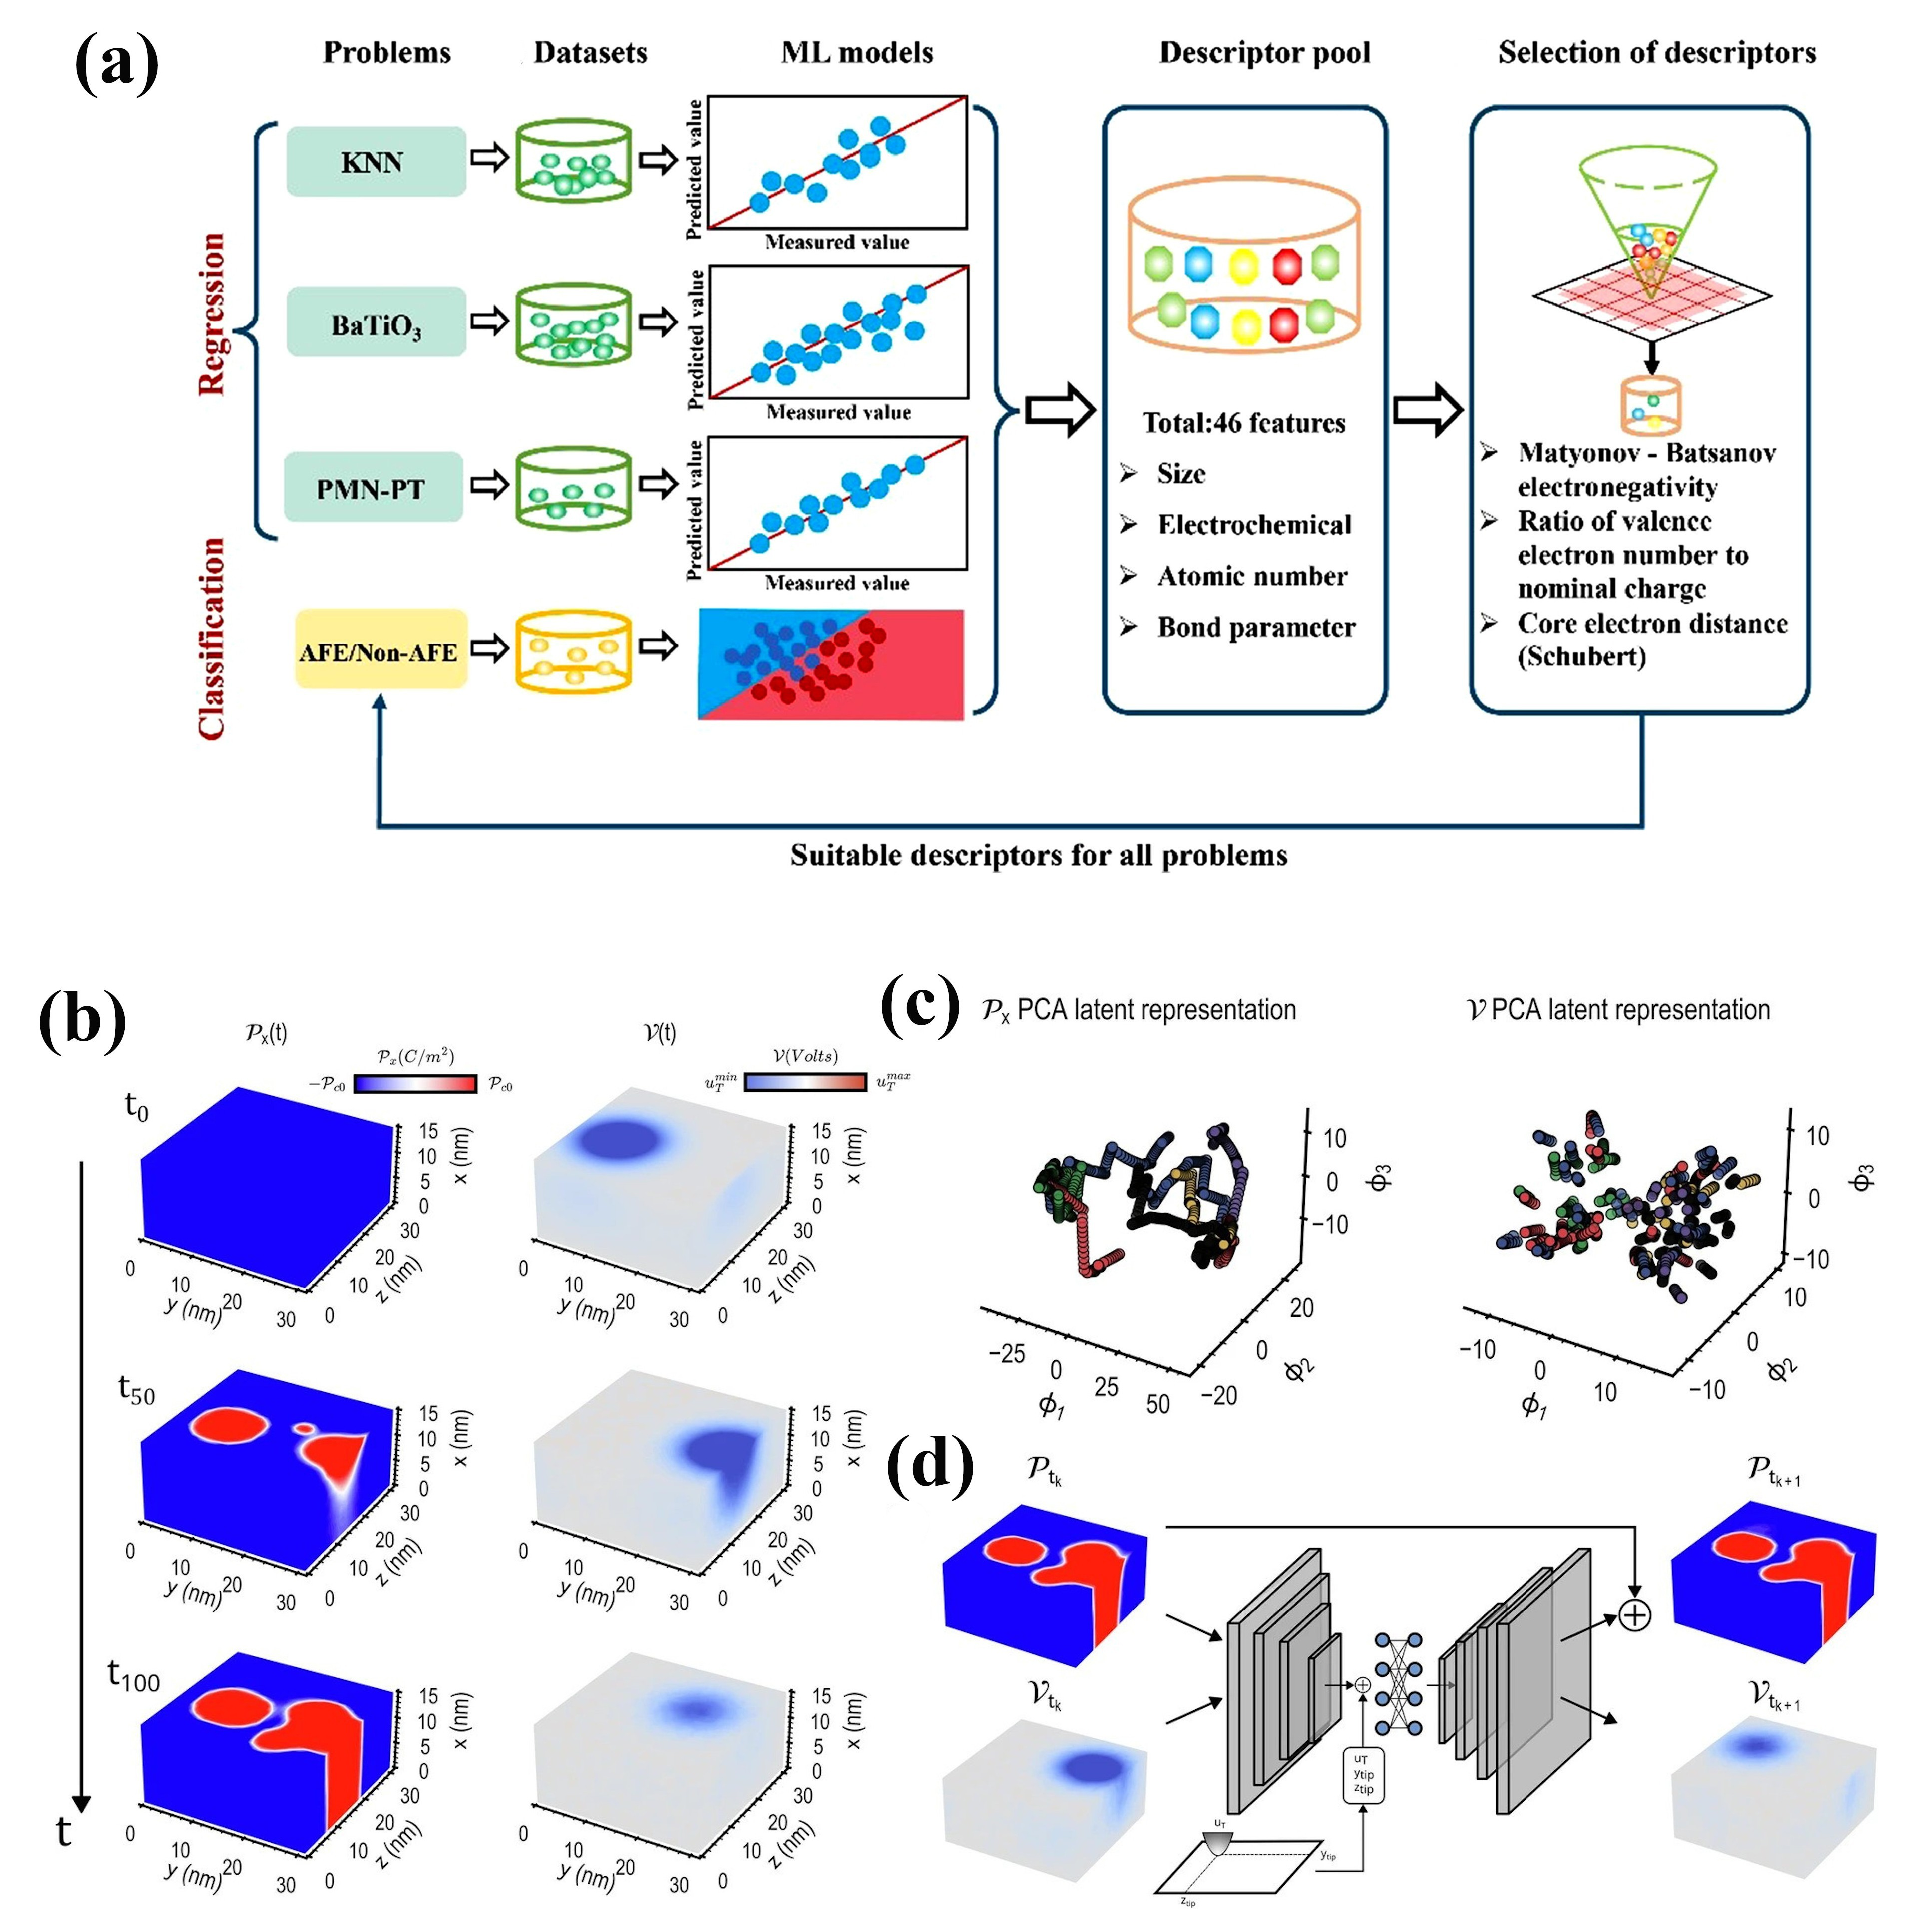
\includegraphics[scale = 0.125]{ml-figure1}\\
\caption{ In order to build a machine learning model on ferroelectric materials, it is necessary to identify the materials descriptors as illustrated in (a). The regression (light turquoise color)  and classification (yellow color) types of problems are designed for the given datasets of different categories (illustrated with similar colors). The descriptor pool is created with all possible numerical fingerprints, and feature selection is performed to ensure relevance to the criteria. The development of surrogate models from phase field method-generated datasets is shown in (b)-(d). The phase field simulations shown in (b) illustrate the spatio-temporal evolution of polarization vector and electrostatic potential. PCA-based latent representation of the data of variables is shown in (b), whereas the ML surrogate model's mapping of the spatio-temporal variables dataset is presented in (c). (The image (a) is reproduced with permission from ~\cite{HE2021116815} and images (b)-(c) are reproduced with permission from ~\cite{Alhada-Lahbabi2024}.)   }
\label{machine-learning-physics1}
\end{figure}%
%%%%%%%%%%%%%%%%%%%%%%%%%%%%%%%%%%%%%%%%%%%%%%%%%%%%%%%%%%%%%%%%%%%%%%%%%%%%%%%%%%%%%%%%%%%%%%%%%%%%%%%%%%%%%%%%%%%%%%%%%%%%%%%%%%%%%%%%%%%%%%%%%%%%%%%%%%%%%%%%%%%%%%%%%%%%%%%%%%%%%%%%%%%%%%%%%%%%%%%%%%%%%%%%%%%%%%%%%%%%%
\section{Multiscale Modeling of Ferroelectricity: From First-Principles to Phase-Field (with Data-Driven Advances)}
\par Ferroelectric materials display spontaneous polarization that can be reversed by external electric fields, allowing for applications in non-volatile memory, actuators, and energy harvesting. Their switching behavior spans from atomic to microscale domains, necessitating multiscale computational approaches for a complete understanding. Density functional theory (DFT) reveals quantum-scale properties, while phase-field methods simulate mesoscale domain dynamics. Integration with machine learning enhances model accuracy and efficiency. Recent advances combine parameters derived from DFT with phase-field models, enabling precise predictions of domain behavior. This review examines multiscale modeling strategies, discusses challenges in scale bridging, and highlights applications in ferroelectric material design. Key focuses include DFT-phase-field integration, data-driven approaches, and their role in advancing ferroelectric technologies.

\subsection{Quantum-Scale Modeling: Density Functional Theory (DFT)}
\par Density Functional Theory (DFT) is widely recognized for its effectiveness in computational chemistry and materials science as a fundamental aspect of investigating ferroelectrics at electronic and atomic scales. Crystal structures, polarization, phase stability, and energy barriers can be predicted with high accuracy using DFT. Notably, the precise description of structural and thermodynamic properties of ferroelectrics achieved by DFT is considered one of its most significant accomplishments \cite{gigli2024modeling}. The spontaneous polarization of a material, lattice instabilities (soft modes), and the contributions of atomic distortions to ferroelectric behavior can be calculated using density functional theory (DFT). Modern advancements, such as Berry phase theory, enable the accurate first-principles computation of polarization and polar discontinuities. The nature of ferroelectric phase transitions has been elucidated through DFT studies, with displacive and order–disorder mechanisms distinguished at the atomic level \cite{liu2014theoretical}. Key material parameters are also provided: for instance, the energy can be mapped as a function of polarization (the 'free energy landscape') using DFT, while domain wall structures and energies are computed, and polarization coupling with strain or electric fields is evaluated. These first-principles insights establish a foundation for higher-scale models.

\par Direct application of density functional theory (DFT) to mesoscale ferroelectric phenomena remains limited by several constraints. The computational intensity of the DFT restricts simulations to small supercells, typically comprising only a few hundred atoms. Simulating large ferroelectric domains or multi-domain configurations at finite temperatures goes beyond the practical limits of DFT. Moreover, small-cell simulations can introduce finite-size artifacts, including spurious depolarization fields and suppressed fluctuations \cite{gigli2024modeling}. Effective models are often derived from density functional theory (DFT), typically involving simplified interactions or coarse-grained Hamiltonians fitted to first-principles results. These models enable simulations at larger length and time scales. For instance, empirical or semi-empirical effective Hamiltonians—sometimes termed "second-principles" models—have been constructed by fitting DFT data. Such models retain essential degrees of freedom (e.g., soft mode coordinates) while higher-energy details are averaged out \cite{liu2014theoretical}. When treated with Monte Carlo or molecular dynamics methods, such models can capture finite-temperature ferroelectric phase transitions and domain phenomena in larger systems. DFT provides the microscopic parameters and mechanistic insights underpinning higher-scale ferroelectric models. Representative DFT-based studies and their contributions to ferroelectric research are summarized in the Table  below.

\subsection{Mesoscale Modeling: Phase-Field Method}
\par At the mesoscale, the phase-field method has been widely adopted for simulating ferroelectric domain formation, evolution, and switching under applied fields or stresses. In this approach, a ferroelectric crystal is described by a spatially continuous order parameter field, represented by the polarization $\mathbf{P}(\mathbf{r})$, which varies across the material. The system's free energy is expressed as a functional of the polarization field, incorporating bulk thermodynamics, gradient energy, electrostatic contributions, and elastic coupling. The Landau-Ginzburg-Devonshire (LGD) free energy is commonly employed as a starting point, utilizing a polynomial expansion in polarization components that preserves crystal symmetry \cite{liu2014theoretical}. For instance, a uniaxial ferroelectric can be modeled using a sixth-order Landau potential:

\begin{equation}
    \mathcal{F} = \alpha P^2 + \beta P^4 + \gamma P^6 + \dotsb,
\end{equation}

where the coefficients $\alpha(T)$, $\beta$, $\gamma$, etc. are selected to replicate the phase transition behavior. The polarization field evolves according to the time-dependent Ginzburg-Landau equation:

\begin{equation}
    \frac{\partial P_i}{\partial t} = -L\frac{\delta\mathcal{F}}{\delta P_i},
\end{equation}

with $L$ being the kinetic coefficient and the functional derivative accounting for all energy contributions. The coefficients may be treated as temperature-dependent (e.g., $\alpha \propto (T-T_0)$) to align with the Curie temperature. Spatial variations of $P$ are penalized by the gradient energy term $\left(\frac{\delta}{2}|\nabla P|^2\right)$, ensuring finite-width domain walls (with a coefficient $\delta$ linked to domain wall energy $\sigma_{\text{dw}}$ and thickness $\ell$). The electric field $\mathbf{E}$, comprising both applied $\mathbf{E}{\text{app}}$ and internal depolarization fields $\mathbf{E}{\text{dep}}$, couples to $P$ through electrostatic terms $\left(-\mathbf{E} \cdot \mathbf{P}\right)$, while strain effects $\epsilon_{ij}$ are incorporated via elastic coupling terms $\left(-\frac{1}{2}c_{ijkl}\epsilon_{ij}\epsilon_{kl} + q_{ijkl}\epsilon_{ij}P_kP_l\right)$ (including piezoelectric $d_{ijk}$ and electrostrictive $Q_{ijkl}$ contributions). The real-time evolution of domain patterns can be simulated by solving the time-dependent Ginzburg-Landau equations $\left(\frac{\partial P_i}{\partial t} = -\Gamma\frac{\delta F}{\delta P_i}\right)$, which govern relaxation dynamics of $\mathbf{P}(\mathbf{r},t)$ toward local free-energy minima."

\par Phase-field modeling is widely used to study ferroelectric phenomena at the mesoscale. This approach effectively captures complex domain structures, including stripe domains and vortex patterns. Moreover, it can simulate domain wall motion caused by electric fields, along with the interactions between domains and defects or grain boundaries. Phase-field simulations have been employed to examine how voids, charged defects, or grain junctions serve as nucleation sites for new domains, influencing the switching field and hysteresis behavior. The method has been expanded to include electromechanical coupling, which is essential for the piezoelectric response, as well as thermal effects relevant to pyroelectric and electrocaloric  studies \cite{volker2011multiscale}. Flexoelectricity---the coupling between polarization \(\mathbf{P}\) and strain gradients \(\nabla \boldsymbol{\epsilon}\)---can be incorporated into phase-field models to investigate non-Ising domain wall structures. Phase-field simulations have shown that even nominally Ising (\(180^\circ\)) domain walls in perovskite ferroelectrics can exhibit Bloch-like (\(\mathbf{P}\) rotating out-of-plane) or N\'eel-like (\(\mathbf{P}\) rotating in-plane) polarization rotations due to flexoelectric effects described by the flexocoupling tensor \(\mathbf{f}_{ijkl}\) in the free energy density \(F = \frac{1}{2}f_{ijkl}P_i \partial_j \epsilon_{kl}\) \cite{gu2014flexoelectricity}. Experimental observations of mixed-character domain walls, which earlier simplified models did not capture, have been explained. When calibrated with appropriate material parameters, the phase-field method functions as a "virtual laboratory" for investigating ferroelectric domain behavior under varying conditions. Key phase-field studies, including those incorporating additional physics such as flexoelectricity and temperature dependence, are summarized in the Table below.

\subsection{Bridging Quantum and Mesoscale Models}
\par Integrating density functional theory (DFT) with phase-field descriptions is crucial for achieving a comprehensive understanding of ferroelectricity. A common approach in this context is sequential multiscale modeling, where data derived from DFT or atomistic simulations at a lower scale is employed to parameterize a higher-scale phase-field model. Practically, this involves extracting Landau coefficients, gradient energy terms, and coupling constants for the phase-field free energy through first-principles calculations or atomistic simulations. For example, the double-well LGD potential of a material can be fitted to ab initio calculations of total energy as a function of homogeneous polarization \cite{liu2014theoretical}. Coefficients such as $\alpha_0$ and $\beta$ can be derived from quantum calculations rather than being determined solely through empirical fitting. Similarly, domain wall energies and widths, computed using density functional theory (DFT) or atomic potentials, can be used to constrain the gradient energy coefficient in phase-field models, ensuring accurate mesoscale representation of wall energetics. For instance, in a prior study, first-principles calculations of 180\degree domain walls in BaTiO$_3$ and PbTiO$_3$ provided domain wall energies that directly informed phase-field parameters \cite{gu2014flexoelectricity}. Linking continuum models to solid quantum-mechanical data improves their predictive accuracy and reduces reliance on adjustable parameters.

\par An alternative approach to bridging density functional theory (DFT) and continuum models involves the use of effective Hamiltonians or coarse-grained representations. In ferroelectrics, a well-known example is the effective lattice Hamiltonian for BaTiO\textsubscript{3}, developed in the 1990s. This model is constructed from localized soft-mode coordinates and was fully parameterized using DFT calculations \cite{liu2014theoretical}. Atomic-scale models, which retain discrete lattice sites, are significantly faster than full density functional theory (DFT), enabling large-scale supercell simulations through extensive Monte Carlo sweeps to resolve phase transitions. Such first-principles-based practical Hamiltonian approaches can be integrated with phase-field modeling to bridge length scales. For example, in a recent multiscale study, thermal hysteresis in \ce{BaTiO3} was investigated by coupling an effective Hamiltonian (simulated via Monte Carlo to incorporate atomic-scale thermal fluctuations) with a phase-field continuum model (governing mesoscale domain evolution) \cite{shao2025understanding}. The ferroelectric phase transition and electrocaloric effect were examined from an atomistic perspective using the effective Hamiltonian and from a mesoscale perspective via the phase-field model. Consistent predictions of polarization versus temperature behavior were obtained from both approaches, aligning with experimental observations \cite{shao2025understanding}. This agreement across scales builds confidence that the models are capturing the actual physics.

\subsection*{Challenges in Multiscale Parameter Transfer}
Despite these successes, bridging scales remains challenging. A key difficulty in sequential approaches lies in the transfer of parameters across disparate scales. Parameters obtained at the nanoscale may not directly translate into effective microscale values, particularly when collective effects or temperature renormalization are considered. For instance, while density functional theory (DFT) typically corresponds to $0\,\text{K}$, phase-field coefficients often describe behavior near room temperature or the Curie temperature ($T_{\text{C}}$), necessitating the renormalization of interaction strengths. Additionally, material properties can be influenced by environment- or size-dependent effects that vary across scales. Careful parameter passing between adjacent scales is required in sequential multiscale methods, posing a challenge when spanning the complete nano-to-macro hierarchy \cite{volker2011multiscale}. Concurrent multiscale coupling---such as directly linking on-the-fly density functional theory (DFT) calculations to continuum solvers---is often deemed impractical for ferroelectrics owing to prohibitive computational costs. To circumvent this limitation, intermediate modeling approaches, such as molecular dynamics (MD) simulations employing specialized ferroelectric force fields (occasionally derived from DFT), have been utilized. These methods facilitate the extraction of dynamical properties and the calibration of phase-field domain kinetics \cite{volker2011multiscale}. Achieving quantitative consistency across various lengths and time scales remains challenging, even with these methods. The table below highlights several notable studies that successfully integrated DFT (or atomistic models) with phase-field approaches, showcasing the techniques employed.
\begin{table}[h]
\centering
\caption{Summary of computational studies on flexoelectric effects in ferroelectrics}
\label{tab:studies}
\begin{tabularx}{\textwidth}{l>{\raggedright\arraybackslash}X>{\raggedright\arraybackslash}X}
\toprule
\textbf{Study (Year)} & \textbf{Approach} & \textbf{Key Contribution} \\
\midrule
Gu \textit{et al.}, 2014 & Phase-field + DFT (domain wall structure) & Showed that $180^\circ$ domain walls in BaTiO$_3$ have mixed Bloch--Néel character due to flexoelectricity. Combined phase-field modeling (with flexoelectric term) and first-principles calculations to identify an intrinsic transverse wall polarization component, explaining features missed by simpler Ising models. \\
\midrule
Zhang \textit{et al.}, 2022 & DFT-calibrated phase-field (domain walls) & Calculated domain wall energies for PbTiO$_3$ and BaTiO$_3$ via DFT and used these values to parameterize the gradient energy coefficient in a phase-field model. Ensured that the continuum model reproduces realistic wall energy and thickness, improving its predictive accuracy for domain patterns. \\
\midrule
Shao \& Huang, 2025 & Effective Hamiltonian + Phase-field (thermal hysteresis) & Employed a first-principles-based effective Hamiltonian (atomistic Monte Carlo) alongside phase-field simulations to study thermal hysteresis in BaTiO$_3$. Both methods consistently reproduced the first-order phase transition and electrocaloric effect, validating a pathway for concurrent multiscale simulation of ferroelectric transitions. \\
\midrule
Others (e.g.\ Li \textit{et al.}, 2016; Liu \textit{et al.}, 2017) & DFT-informed Landau theory (sequential) & Derived Landau-Devonshire polynomial coefficients from first-principles calculations (or bolstered by MD) for specific ferroelectrics. Enhanced phase-field models of devices (e.g.\ thin-film capacitors) by using DFT-based dielectric and piezoelectric constants, improving agreement with experiments. (References in text) \\
\bottomrule
\end{tabularx}
\end{table}


%%%%%%%%%%%%%%%%%%%%%%%%%%%%%%%%%%%%%%%%%%%%%%%%%%%%%%%%%%%%%%%%%%%%%%%%%%

\section{Highlights on Energy Harvesting Applications of Ferroelectric Materials}\label{results_discussions}
\begin{enumerate}
    \item Thermal Energy
    \item Solar Energy
    \item Harvesting stray magnetic field
    \item Electric energy storage with (Pb-based/Pb-free) ferroelectric ceramic capacitors
\end{enumerate}

\section{Advancing the application potentials of ferroelectric devices with AI techniques} \label{emergent_technology}



%\subsection{Undertainty Quantification and AI} \label{optimization}

\section{Conclusions}\label{conclusions}
Conclusions related to positive results.

\section*{Declaration of Competing Interests}
The authors declare that they have no known competing financial interests or personal relationships that could have appeared to influence the work reported in this paper.

% \section*{CRediT author statement}
% \textbf{}: Conceptualization, Methodology, Software, Validation, Investigation, Formal Analysis, Data Curation, Visualization,  Writing - Original Draft. \textbf{}: Methodology, Formal Analysis, Validation, Writing- Reviewing and Editing. \textbf{}: Validation, Software, Visualization, Formal Analysis, Writing- Reviewing and Editing. \textbf{}:  Methodology, Validation, Supervision, Writing- Reviewing and Editing. \textbf{}: Formal Analysis, Validation, Writing- Reviewing and Editing. \textbf{}: Conceptualization, Methodology, Supervision, Validation,  Data Curation, Funding acquisition, Project administration, Writing- Reviewing and Editing.

\section*{Acknowledgments}
 This work was supported by the National Science Centre, Poland (UMO-2021/42/E/ST5/00339). 
 
 
\section*{Availability of data and materials}
The data and codes for this study are available in \url{https://github.com/anilkunwar/ferroelectric_materials2025}
% \section*{Supplementary material}

% The supplementary material is attached.





% \end{document}


%Two bibliographic style files (\verb+*.bst+) are provided ---
%{model1-num-names.bst} and {model2-names.bst} --- the first one can be
%used for the numbered scheme. This can also be used for the numbered
%with new options of {natbib.sty}. The second one is for the author year
%scheme. When  you use model2-names.bst, the citation commands will be
%like \verb+\citep+,  \verb+\citet+, \verb+\citealt+ etc. However, when
%you use model1-num-names.bst, you may use only \verb+\cite+ command.

%\verb+thebibliography+ environment.  Each reference is a
%\verb+\bibitem+ and each \verb+\bibitem+ is identified by a label,
%by which it can be cited in the text:

%\noindent In connection with cross-referencing and
%possible future hyperlinking it is not a good idea to collect
%more that one literature item in one \verb+\bibitem+.  The
%so-called Harvard or author-year style of referencing is enabled
%by the \LaTeX{} package {natbib}. With this package the
%literature can be cited as follows:


%\begin{enumerate}[\textbullet]
%\item Parenthetical: \verb+\citep{WB96}+ produces (Wettig \& Brown, 1996).
%\item Textual: \verb+\citet{ESG96}+ produces Elson et al. (1996).
%\item An affix and part of a reference:
%\verb+\citep[e.g.][Ch. 2]{Gea97}+ produces (e.g. Governato et
%al., 1997, Ch. 2).
%\end{enumerate}

%In the numbered scheme of citation, \verb+\cite{<label>}+ is used,
%since \verb+\citep+ or \verb+\citet+ has no relevance in the numbered
%scheme.  {natbib} package is loaded by {cas-sc} with
%\verb+numbers+ as default option.  You can change this to author-year
%or harvard scheme by adding option \verb+authoryear+ in the class
%loading command.  If you want to use more options of the {natbib}
%package, you can do so with the \verb+\biboptions+ command.  For
%details of various options of the {natbib} package, please take a
%look at the {natbib} documentation, which is part of any standard
%\LaTeX{} installation.



%\printcredits

\printcredits



%% Loading bibliography style file
\bibliographystyle{model1-num-names}
%\bibliographystyle{model2-names}

% Loading bibliography database
% \bibliography{refs}
%\bibliography{./home/username/Documents/my_bib_files/reactive_wetting2018}
%\bibliography{./../../../../../../Documents/my_bib_files/electromigration_reference}
%\bibliography{./../../../../../../../../Documents/my_bib_files/electromigration_reference}
%\bibliography{/home/username/Documents/my_bib_files/electromigration_reference}
%\bibliography{electromigration_reference}
%\bibliography{./../../../../../../Documents/my_bib_files/refs}
%\bibliography{/home/username/Documents/electromigration_reference}
%\bibliography{thermomigration_reference}
\bibliography{ferroelectricmaterials_reference}

% \newpage
\appendix
\renewcommand{\thesection}{Appendix \Alph{section}}

%%%%%%%%%%%%%%%%%%%%%%%%%%%%%%%%%%%%%%%
% Set numbering scheme for tables to "A.1"
\numberwithin{table}{section}
% \renewcommand\thetable{\thesection.\arabic{table}}
\renewcommand{\thetable}{\Alph{section}.\arabic{table}}
%%%%%%%%%%%%%%%%%%%%%%%%%%%%%%%%%%%%%%%%%%%%%%%%%%%%%%%%
%%%%%%%%%%%%%%%%%%%%%%%%%%%%%%%%%%%%%%%%%%%%%%%%%%%%%%%%
\numberwithin{equation}{section}
% \renewcommand{\theequation}{\thesection.\arabic{equation}}
\renewcommand{\theequation}{\Alph{section}.\arabic{equation}}
% Customize equation numbering format



\iffalse

\section{Appendix }



\fi



%\verb+\printcredits+ command is used after appendix sections to list 
%author credit taxonomy contribution roles tagged using \verb+\credit+ 
%in frontmatter.
%\end{multicols}
\end{document} 

